% % !Mode:: "TeX:UTF-8"
% % !TEX builder = LATEXMK
% % !TEX program = xelatex
% \documentclass[master,twoside,nocpsupervisor]{zjuthesis}

% % 插图路径设置,图片放在figures 文件夹下。一般来说论文的插图比较多,通常按章节存
% % 放,因此可以在以下命令中在按章节添加存放图片的文件夹路径。如以下这个路径中 ./
% % 代表当前main.tex所在的目录,就是一般所说的当前文件夹;figures 文件夹就是子文件
% % 夹,存放正文及附录中要用到的所有的图片,在figures 文件夹中的子文件夹就是存放各
% % 个章节图片的文件夹,一般命名与相应章节的名字相同,如intro 章节用到的图片全放在
% % 了intro 这个子文件夹下。
% \graphicspath{%
% 	{./figures/intro/}%
% }

% % 论文中文标题
% \title{浙江大学研究生学位论文编写规则\LaTeX 模板}
% % 论文英文标题
% \englishtitle{Workspace control system of underwater tele-operated manipulators on an ROV}
% % 作者,就是你的名字
% \author{Monster,Hamburger}
% % 分类号
% \classification{TM863}
% % 单位代码
% \serialnumber{10335}
% % 密级
% \secretlevel{公开}
% % 学号
% \studentnumber{12312345}
% % 指导教师
% \supervisor{诸葛亮}
% % 合作导师,如果没有合作导师,就在\documentclass选项栏中加上"nocpsupervisor"。
% \cpsupervisor{庞统}
% % 专业名称
% \major{武器制造}
% % 研究方向
% \research{木牛流马研究}
% % 所在学院
% \institute{机械工程学院}
% % 提交日期
% \submitdate{225年1月1日}

% % 中文题名页
% \reviewerA{关羽\hspace{1.5em}五虎上将\hspace{1.5em}蜀汉}
% \reviewerB{张飞\hspace{1.5em}五虎上将\hspace{1.5em}蜀汉}
% \reviewerC{马超\hspace{1.5em}五虎上将\hspace{1.5em}蜀汉}
% \reviewerD{黄忠\hspace{1.5em}五虎上将\hspace{1.5em}蜀汉}
% \reviewerE{赵云\hspace{1.5em}五虎上将\hspace{1.5em}蜀汉}
% \chairperson{许攸\hspace{1.5em}文臣谋士\hspace{1.5em}曹魏}
% \commissionerA{法正\hspace{1.5em}文臣谋士\hspace{1.5em}蜀汉}
% \commissionerB{简雍\hspace{1.5em}文臣谋士\hspace{1.5em}蜀汉}
% \commissionerC{麋竺\hspace{1.5em}文臣谋士\hspace{1.5em}蜀汉}
% \commissionerD{孙乾\hspace{1.5em}文臣谋士\hspace{1.5em}蜀汉}
% \commissionerE{伊籍\hspace{1.5em}文臣谋士\hspace{1.5em}蜀汉}
% \defencedate{225年3月5日}

% % 英文题名页
% \enreviewerA{Guan Yu\hspace{1.5em} general \hspace{1.5em} Shu-Han}
% \enreviewerB{Zhang Fei\hspace{1.5em} general \hspace{1.5em} Shu-Han}
% \enreviewerC{Ma Chao\hspace{1.5em} general \hspace{1.5em} Shu-Han}
% \enreviewerD{Huang Zhong\hspace{1.5em} general \hspace{1.5em} Shu-Han}
% \enreviewerE{Zhao Yun\hspace{1.5em} general \hspace{1.5em} Shu-Han}
% \enchairperson{Xu You \hspace{1.5em} counsellor \hspace{1.5em} Cao Wei}
% \encommissionerA{Fa Zheng \hspace{1.5em} counsellor \hspace{1.5em} Shu-Han}
% \encommissionerB{Jian Yong \hspace{1.5em} counsellor \hspace{1.5em} Shu-Han}
% \encommissionerC{Mi Zhu \hspace{1.5em} counsellor \hspace{1.5em} Shu-Han}
% \encommissionerD{Sun Gan \hspace{1.5em} counsellor \hspace{1.5em} Shu-Han}
% \encommissionerE{Yi Ji \hspace{1.5em} counsellor \hspace{1.5em} Shu-Han}
% \eendefencedate{March 5, 225}

% \begin{document}
% \maketitle
% % \ZJUmakecover
% % \ZJUmakeCNtitlepage
% % \ZJUmakeENtitlepage
% \frontmatter
% % !TEX root = ../main.tex
\chapter{致\texorpdfstring{\ZJUspace}{}谢}
岁月如梭,转眼间,X年的XX生求学生活即将结束,站在毕业的门槛上,回首往昔,奋斗和辛劳成为丝丝的记忆,甜美与欢笑也都尘埃落定。浙江大学以其优良的学习风气、严谨的科研氛围教我求学,以其博大包容的情怀胸襟、浪漫充实的校园生活育我成人。值此毕业论文完成之际,我谨向所有关心、爱护、帮助我的人们表示最诚挚的感谢与最美好的祝愿。

本论文是在导师诸葛亮丞相的悉心指导之下完成的。三年来,导师渊博的专业知识,严谨的治学态度,精益求精的工作作风,诲人不倦的高尚师德,朴实无华、平易近人的人格魅力对我影响深远。导师不仅授我以文,而且教我做人,虽历时X载,却赋予我终生受益无穷之道。本论文从选题到完成,几易其稿,每一步都是在导师的指导下完成的,倾注了导师大量的心血,在此我向我的导师诸葛丞相表示深切的谢意与祝福!

本论文的完成也离不开其他各位老师、同学和朋友的关心与帮助。在此也要感谢关羽、赵云等各位老师在论文开题、初稿、预答辩期间所提出的宝贵意见,感谢木牛流马课题组为本论文提供的数据和建议,还要感谢同门的师兄师妹们,在科研过程中给我以许多鼓励和帮助。回想整个论文的写作过程,虽有不易,却让我除却浮躁,经历了思考和启示,也更加深切地体会了法学的精髓和意义,因此倍感珍惜。

还要感谢父母在我求学生涯中给与我无微不至的关怀和照顾,一如既往地支持我、鼓励我。同时,还要感谢关某某同学、赵某某同学、张某某同学、黄某某同学X年来对我的爱护、包容和帮助,愿友谊长存!

\vspace{2cm}
\hfill
\begin{minipage}{14em}
\begin{center}
于XX地\quad 225年1月1日\\
我的名
\end{center}
\end{minipage}

% % !TEX root = ../main.tex

% 定义中文摘要和关键字
\begin{cabstract}
请注意,以下内容是参考自\textbf{薛瑞尼}的清华大学论文模板,主要是为了填内容方便。

论文的摘要是对论文研究内容和成果的高度概括。摘要应对论文所研究的问题及其研究目
的进行描述,对研究方法和过程进行简单介绍,对研究成果和所得结论进行概括。摘要应
具有独立性和自明性,其内容应包含与论文全文同等量的主要信息。使读者即使不阅读全
文,通过摘要就能了解论文的总体内容和主要成果。

论文摘要的书写应力求精确、简明。切忌写成对论文书写内容进行提要的形式,尤其要避
免“第 1 章……;第 2 章……;……”这种或类似的陈述方式。

本文介绍浙江大学论文模板的使用方法。本模板符合学校的硕士、博士论文格式要求。
写这个模板的主要原因是想深入学习一下\LaTeX,还有可以自己毕业的时候用。

本文的创新点主要有:
\begin{itemize}
	\item 用例子来解释模板的使用方法;
	\item 用废话来填充无关紧要的部分;
	\item 一边学习摸索一边编写新代码。
\end{itemize}

关键词是为了文献标引工作、用以表示全文主要内容信息的单词或术语。关键词不超过 5
个,每个关键词中间用分号分隔。(模板作者注:关键词分隔符不用考虑,模板会自动处
理。英文关键词同理。)
\end{cabstract}

\ckeywords{\TeX, \LaTeX, CJK, 模板, 毕业论文}

% % !TEX root = ../main.tex

% 定义英文摘要和关键字

\begin{eabstract}
An abstract of a dissertation is a summary and extraction of research work
and contributions. Included in an abstract should be description of research
topic and research objective, brief introduction to methodology and research
process, and summarization of conclusion and contributions of the
research. An abstract should be characterized by independence and clarity and
carry identical information with the dissertation. It should be such that the
general idea and major contributions of the dissertation are conveyed without
reading the dissertation.

An abstract should be concise and to the point. It is a misunderstanding to
make an abstract an outline of the dissertation and words ``the first
chapter'', ``the second chapter'' and the like should be avoided in the
abstract.

Key words are terms used in a dissertation for indexing, reflecting core
information of the dissertation. An abstract may contain a maximum of 5 key
words, with semi-colons used in between to separate one another.
\end{eabstract}

\ekeywords{\TeX, \LaTeX, CJK, template, thesis}

% % 正文目录:
% \tableofcontents
% % 插图目录:
% \listoffigures
% % 表格目录:
% \listoftables
% % !TEX root = ../main.tex
\begin{denotation}

\item[HPC] 高性能计算 (High Performance Computing)
\item[cluster] 集群
\item[Itanium] 安腾
\item[SMP] 对称多处理
\item[API] 应用程序编程接口
\item[PI]	聚酰亚胺
\item[MPI]	聚酰亚胺模型化合物,N-苯基邻苯酰亚胺
\item[PBI]	聚苯并咪唑
\item[MPBI]	聚苯并咪唑模型化合物,N-苯基苯并咪唑
\item[PY]	聚吡咙
\item[PMDA-BDA]	均苯四酸二酐与联苯四胺合成的聚吡咙薄膜均苯四酸二酐与联苯四胺合成的聚吡咙薄膜均苯四酸二酐与联苯四胺合成的聚吡咙薄膜
\item[$\Delta G$]  	活化自由能~(Activation Free Energy)
\item [$\chi$] 传输系数~(Transmission Coefficient)
\item[$E$] 能量
\item[$m$] 质量
\item[$c$] 光速
\item[$P$] 概率
\item[$T$] 时间
\item[$v$] 速度
\end{denotation}

% \mainmatter
% % !TEX root = ../main.tex

\chapter{绪论\texorpdfstring{\footnote{章标题中脚注命令测试}}{}(or 引言)各种测试}
绪论占坑,但是也要测试到底占多少缩进,换行情况,行距,都是这些不听话的小伙伴,好好调教你们。

\section{列表环境\texorpdfstring{\footnote{节标题中脚注命令测试}}{}测试}
以下是一个测试用的列表环境,内容不要在意。\footnote{正文中中脚注命令测试,长脚注情况:这包括如下事实:“未经本人同意,监听、录制或转播私人性质的谈话或秘密谈话;未经本人同意,拍摄、录制或转播个人在私人场所的形象”}

这里测试列表标签功能的交叉引用格式\ref{itm:11},\ref{itm:12},\ref{itm:13},\ref{itm:14},分别表示第一至第四层级的itemize系列的交叉引用情况。
\begin{enumerate}
	\item 第一级列表\label{itm:11}
	\item 第一级列表
	\begin{enumerate}
		\item 第二级列表\label{itm:12}
		\item 第二级列表
		\begin{enumerate}
			\item 第三级列表\label{itm:13}
			\item 第三级列表
			\begin{enumerate}
				\item 第四级列表\label{itm:14}
				\item 第四级列表
				\item 第四级列表
				\item 第四级列表
			\end{enumerate}
			\item 第三级列表
			\item 第三级列表
			\item 第三级列表
		\end{enumerate}
		\item 第二级列表
		\item 第二级列表
	\end{enumerate}
	\item 第一级列表
	\item 第一级列表
	\item 第一级列表
\end{enumerate}

正是由于油膜物质的发现,使“雾伞”计划成为可能,这个计划是用核爆炸在太空中蒸发和扩散油膜物质,在太阳与地球之间形成一团“油膜尘埃”,降低太阳 对地球的辐射,达到缓解地球温室效应的目的。“我记得,海王星轨道附近应该还有前战争时期的恒星型核弹吧?”肯又问。“有的,‘雾伞’工程的飞船也装载了一些,在海王星环和卫星上爆破用,具体数目不清楚。” “好像一颗就够了。”肯兴奋起来。两个世纪前面壁者雷迪亚兹的战略计划中所研制的恒星型氢弹,后来共制造了五千多颗。虽然这种武器在末日之战中作用有限,但正如雷迪亚兹所言,各大 国主要是为可能爆发的人类之间的行星际战争准备的,核弹主要在大低谷时期制造,那时由于资源的匮乏,国际关系极其紧张,人类自身的战争一触即发。进入新时期后,这些骇人听闻的武器成了危险的鸡肋,虽然其所有权都属于地球国家, 但还是都被送入太空存贮,少部分已经用于行星工程的爆破,还有一部分送入太阳系外围轨道。曾有人设想将核弹中的聚变材料可以作为远程飞船的燃料补充,但由于核弹的拆解很困难,这个设想一直没有真正实现过\footnote{看看另起一页脚注编号的变化}。
\begin{itemize}
	\item 第一级列表
	\item 第一级列表
	\begin{itemize}
		\item 第二级列表
		\item 第二级列表
		\begin{itemize}
			\item 第三级列表
			\item 第三级列表
			\begin{itemize}
				\item 第四级列表
				\item 第四级列表
				\item 第四级列表
				\item 第四级列表
			\end{itemize}
			\item 第三级列表
			\item 第三级列表
			\item 第三级列表
		\end{itemize}
		\item 第二级列表
		\item 第二级列表
	\end{itemize}
	\item 第一级列表
	\item 第一级列表
	\item 第一级列表
\end{itemize}

“你觉得能行,”罗宾逊两眼放光地问道,他后悔这么简单的事自己怎么没 想到,一个载入史册的机会让肯抢去了。“试试吧,只有这一个办法了。”“如果行,博士,以后林格一斐兹罗监测站将永远按产生1G重力的速度旋转。”“这可是人类造出来的最大的东西了。”“蓝影”号飞船的指令长看着舱外漆黑的太空说,他极力想象自己能看到尘埃云,但确实什么\footnote{连续两个脚注测试1}\footnote{连续两个脚注测试2}
\begin{enumerate}
	\item 第四级列表
	\item 第四级列表
	\begin{enumerate}
		\item 第五级列表
		\item 第五级列表
		\item 第五级列表
	\end{enumerate}
	\item 第四级列表
	\item 第四级列表
\end{enumerate}
都看不到。“为什么它不能被阳光照出来呢,就像彗星的尾巴那样...”飞船驾驶员说,“蓝影”号上只有他和指令长两个人。他知道,尘埃云的密度确实像彗星尾一样稀薄,几乎和地球上实验室中造出的真空差不多。“可能是阳光太弱吧。”指令长回头看看太阳,在这海王星轨道和柯伊伯带 之间的冷寂空间,太阳看上去只是一颗刚能看出圆盘形状的大星星。阳光倒是还可以在舱壁上照出亮影,但已经十分微弱了。“再说,彗尾也要在一定的距离外 才能看到,我们可是就在云的边缘。”

\section{参考文献测试}
测试一下引用\cite{shi_chinas_2010},引用\cite{shi2010china,hata2014soi,muhammad2011development},还有其它引用\cite{shi2010china,muhammad2011development,lamport1994latex}.

\section{浮动体测试}
\subsection{插图测试}
如\autoref{fig:first_image_tset}是对此模版的第一张插图测试。

\begin{figure}[htbp]
	\centering
	
\includegraphics[width = 0.5\linewidth]{Chapter1.png}
	\caption{第一张插图测试}\label{fig:first_image_tset}
\end{figure}

以下是一段对这些插图来历的介绍,引用自知乎专栏All about TeXnique中夏晓昊的文章\href{http://zhuanlan.zhihu.com/LaTeX/19669122}{《The TeXbook导读:从那头(多图杀猫的)狮子说起》}。

在The TeXbook中,有着一系列的以狮子为主题的插图。这些插图的作者是Duane Bibby。也是从The TeXbook开始,不少TeX书也采取了以狮子为主的插图,作者也是Duane Bibby。另外,每年的TUG(TeX Users Group)年会都会有一张以狮子为主题的logo,这只狮子已经是社区的吉祥物了。

为什么选择狮子呢?Yannis Haralambous写道(原文法语,此为转译后的英文):Not for nothing is TeX represented by a lion. Donald Knuth has told us that lions are to him the guardians of libraries in the United States because there is a statue of a lion in front of the entrance of each large library there. Guardian of libraries, guardian of the Book—is that not indeed what TeX ultimately aspires to be? 或许吧。 (顺便说一句,TeX和MetaFont都用了狮子,TeX是公狮子,MetaFont是母狮子,多么和谐的一对啊。如果你还是忽略MetaFont的存在,那你还没有认识到它的重要性。)

作为插图,首要的一点就是贴切,然后是有趣。在TeX社区里面,have fun是一个很重要的词组,也有人说Happy TeXing。我知道有不少人不喜欢TeX,但是能有什么理由呢?如果你用不到它,那么浅尝辄止即可。如果你会用到很频繁,最好慢慢修炼做到精通。如果你只是偶尔用到,那么可以搬个模版什么的,甚至也可以找人帮你(不要指望别人会用足够的空闲时间来帮你,他没有这个义务,请支付报酬,最少也得请吃个红烧肉吧)。下面的插图,是TeX TeXbook中的,我也希望这个新年的假期,能有人有空来看看这本书。即使不能把所有的东西都看懂,那么也会对TeX的设计有了一定的了解,拿到扳手就好。

\subsection{表格测试}
在这里推荐制表采用功能强大的tabu宏包以取代其它制表宏包。具体tabu宏包的使用说明参见tabu宏包的说明文档。

以下节分别用来测试各种表格环境如,tabular,tabu,longtabu等,还有对caption格式的修改和测试。以下表格样式全部采用三线表。

\subsubsection{array宏包tabular表格环境测试}
如\autoref{tab:first_table_test}是对array宏包的tabular表格环境测试。
\begin{table}[htbp]
	\centering
	\caption{这是一个用tabular环境的测试用的表格}\label{tab:first_table_test}
    \begin{tabular}{lrr}
    \toprule
    \textbf{行星}     & \textbf{赤道半径}km & \textbf{公转周期}d \\
    \midrule
    水星     & 2.439  & 87.9 \\
    金星     & 6.1    & 224.682 \\
    地球     & 6378.14 & 365.24 \\
    \bottomrule
    \end{tabular}%
\end{table}

\subsubsection{tabu宏包表格环境测试}
如\autoref{tab:tabu_test_1}是对tabu宏包的tabu表格环境测试。在这里表格命令与\autoref{tab:first_table_test}的命令相同,只是tabular环境改成了tabu环境。
\begin{table}[htbp]
	\centering
	\caption{这是一个用tabu环境的测试用的表格}\label{tab:tabu_test_1}
    \begin{tabu}{lrr}
    \toprule
    \textbf{行星}     & \textbf{赤道半径}km & \textbf{公转周期}d \\
    \midrule
    水星     & 2.439  & 87.9 \\
    金星     & 6.1    & 224.682 \\
    地球     & 6378.14 & 365.24 \\
    \bottomrule
    \end{tabu}%
\end{table}

\autoref{tab:tabu_test_2}对tabu to表格的x列模式进行测试。在表格导言区中设置为X[1]X[2]X[2],表示这三列表格的列宽比值为1:2:2,总的表格宽度由tabu to环境设置,这里设置为0.6\textbackslash linewidth。相比于tabular环境,tabu环境的列宽设置方便许多。
\begin{table}[htbp]
	\centering
	\caption{tabu环境测试表格---X列模式}\label{tab:tabu_test_2}
    \begin{tabu} to 0.6\linewidth{X[1]X[2]X[2]}
    \toprule
    \textbf{行星}     & \textbf{赤道半径}km & \textbf{公转周期}d \\
    \midrule
    水星     & 2.439  & 87.9 \\
    金星     & 6.1    & 224.682 \\
    地球     & 6378.14 & 365.24 \\
    \bottomrule
    \end{tabu}%
\end{table}

如\autoref{tab:tabu_test_3}是longtabu环境测试表格。longtabu环境不能用在table浮动体环境中。根据GB/T 7713.1-2006规定:如果某个表需要转页接排,在随后的各页上应重复表的编号。编号后跟标题(可省略)和“(续)”,置于表上方。续表应重复表头。

特别需要注意的是,longtabu是基于longtable宏包开发的,所以在zjuthesis.cls文件中已经插入了longtable宏包。longtable环境的所有功能都可以在longtabu中使用,如\textbackslash endhead,\textbackslash endfirsthead,\textbackslash endfoot,\textbackslash endlastfoot,和\textbackslash caption等。具体用法请参见longtable和tabu宏包的相应文档。
\begin{longtabu}{lccc}
\caption{材料弹性模量及泊松比}\label{tab:tabu_test_3}\\
\toprule
名  称   & 弹性模量E/Gpa & 切变模量G/Gpa & 泊松比$\mu$ \\
\midrule%
\endfirsthead
\caption{材料弹性模量及泊松比(续)}\\
\toprule
名  称   & 弹性模量E/Gpa & 切变模量G/Gpa & 泊松比$\mu$ \\
\midrule%
\endhead
\bottomrule%
\endfoot
镍铬钢、合金钢 & 206    & 79.38  & 0.3 \\
碳 钢    &  196~206 & 79     & 0.3 \\
铸 钢    &  172~202 &        & 0.3 \\
球墨铸铁   &  140~154 &  73~76 & 0.3 \\
灰铸铁、白口铸铁 &  113~157 & 44     &  0.23~0.27 \\
冷拔纯铜   & 127    & 48     &   \\
轧制磷青铜  & 113    & 41     &  0.32~0.35 \\
轧制纯铜   & 108    & 39     &  0.31~0.34 \\
轧制锰青铜  & 108    & 39     & 0.35 \\
铸铝青铜   & 103    & 41     & 0.3 \\
冷拔黄铜   &  89~97 &  34~36 &  0.32~0.42 \\
轧制锌    & 82     & 31     & 0.27 \\
硬铝合金   & 70     & 26     & 0.3 \\
轧制铝    & 68     &  25~26 &  0.32~0.36 \\
铅      & 17     & 7      & 0.42 \\
玻璃     & 55     & 22     & 0.25 \\
混凝土    &  14~39 &  439~15.7 &  0.1~0.18 \\
纵纹木材   &  9.8~12 & 0.5    &   \\
横纹木材   &  0.5~0.98 &  0.44~0.64 &   \\
橡胶     & 0.00784 &        & 0.47 \\
电木     &  1.96~2.94 &  0.69~2.06 &  0.35~0.38 \\
赛璐珞    &  1.71~1.89 &  0.69~0.98 & 0.4 \\
可锻铸铁   & 152    &        &  \\
拔制铝线   & 69     &        &  \\
大理石    & 55     &        &  \\
花岗石    & 48     &        &  \\
石灰石    & 41     &        &  \\
尼龙1010 & 1.07   &        &  \\
夹布酚醛塑料 &  4~8.8 &        &  \\
石棉酚醛塑料 & 1.3    &        &  \\
高压聚乙烯  &  0.15~0.25 &        &  \\
低压聚乙烯  &  0.49~0.78 &        &  \\
聚丙烯    &  1.32~1.42 &        &  \\
硬聚氯乙烯  &  3.14~3.92 &        &  \\
聚四氟乙烯  &  1.14~1.42 &        &  \\
\end{longtabu}%

\subsection{子图}
这里子图的排版推荐使用subcaption宏包,不再推荐使用subfig宏包,更不推荐使用subfigure宏包。值得注意的是,在zjuthesis.cls文件中已经写入了subcaption宏包,而且subcaption宏包与subfigure和subfig宏包是相互冲突的。因此,如果你还想使用subfig宏包而不想使用subcaption宏包,请自己到zjuthesis.cls文件的相关位置更改,具体的使用及修改方法参见相应的宏包说明文档。不过在这里还是不推荐直接去更改zjuthesis.cls文档,除非你对\LaTeX 的相关命令很清楚,知道自己在改什么,并且不会对其他格式产生影响。

具体的subcaption宏包使用方法我这里不仔细介绍,以下只是对subcaption进行一些简单的测试,主要是格式调整和交叉引用。

如\autoref{fig:subfig_test1}是有两张子图的模式,对子图进行交叉引用,如\autoref{subfig:1a}和\autoref{subfig:1b}。

\begin{figure}[htbp]
	\centering
	\begin{subfigure}[b]{.4\textwidth}
		\centering
		
\includegraphics[width = \textwidth]{Chapter2.png}
		\caption{书籍排版与普通排版}\label{subfig:1a}
	\end{subfigure}
	\quad
	\begin{subfigure}[b]{.4\textwidth}
		\centering
		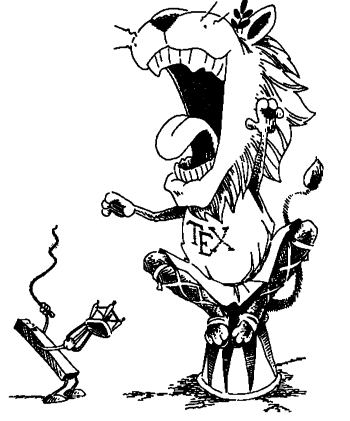
\includegraphics[width = \textwidth]{Chapter3.png}
		\caption{\TeX 的控制系列}\label{subfig:1b}
	\end{subfigure}
	\caption{子图模式测试1:2张图}\label{fig:subfig_test1}
\end{figure}

如\autoref{fig:subfig_test2}是有四张子图的模式,对子图进行交叉引用,如\autoref{subfig:2a}、\autoref{subfig:2b}、\autoref{subfig:2c}和\autoref{subfig:2d}。

\begin{figure}[htbp]
	\centering
	\begin{subfigure}[b]{.4\textwidth}
		\centering
		
\includegraphics[width = \textwidth]{Chapter4.png}
		\caption{字体}\label{subfig:2a}
	\end{subfigure}
	\begin{subfigure}[b]{.4\textwidth}
		\centering
		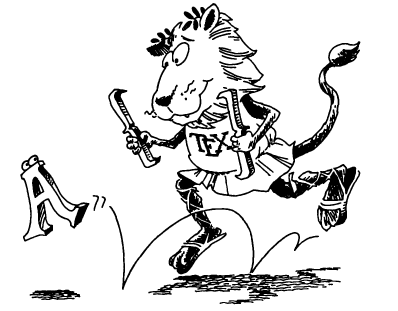
\includegraphics[width = \textwidth]{Chapter5.png}
		\caption{编组}\label{subfig:2b}
	\end{subfigure}
	\begin{subfigure}[b]{.4\textwidth}
		\centering
		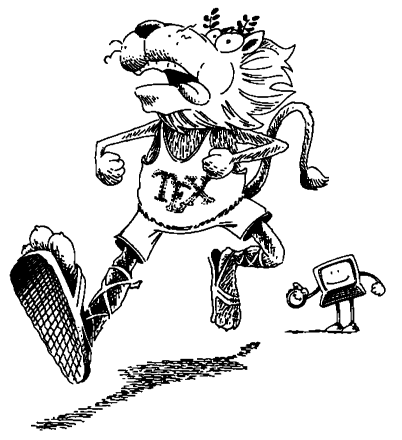
\includegraphics[width = \textwidth]{Chapter6.png}
		\caption{运行\TeX}\label{subfig:2c}
	\end{subfigure}
	\begin{subfigure}[b]{.4\textwidth}
		\centering
		
\includegraphics[width = \textwidth]{Chapter7.png}
		\caption{\TeX 工作原理}\label{subfig:2d}
	\end{subfigure}
	\caption{子图模式测试2:4张图}\label{fig:subfig_test2}
\end{figure}

\subsection{数学模式测试}
数学模式测试,主要测试数学字体,编号和交叉引用。这里首先推荐使用\texttt{align}和\texttt{align*}数学模式环境,大多数行间数学模式只需要用这个环境就可以了。

交叉引用测试,如交引用命令{\ttfamily \textbackslash eqref}和\texttt{\textbackslash ref}命令的区别。如公式\eqref{eq:test1},公式\ref{eq:test1}显示,\texttt{\textbackslash eqref}命令比\texttt{\textbackslash ref}命令的应用结果多了个括号。

如公式\eqref{eq:test3}是单行公式环境,查看公式\eqref{eq:test3}和\eqref{eq:test1}之间的区别,好像在单行公式中没什么区别。
\begin{align}\label{eq:test3}
	f(x) = 2(x + 1)^{2} - 1
\end{align}

\texttt{align}公式环境,用在单行中。
\begin{align}\label{eq:test1}
	f(x) = 2(x + 1)^{2} - 1
\end{align}

在这里,中间插入一些文字以形成段落,查看行间公式与上下文之间的间隙。
\begin{align*}
	f(x) = 2(x + 1)^{2} - 1
\end{align*}
在这里,中间插入一些文字以形成段落,查看行间公式与上下文之间的间隙。下一个公式\eqref{eq:test2}是一个公式组,它在“=”位置对齐。
\begin{align}\label{eq:test2}
	f(x) & = 2(x + 1)^{2} - 1\\
		 & = 2(x^{2} + 2x +1)-1\\
		 & = 2x^{2} + 4x + 1
\end{align}


\section{关于引用}
图表的引用通过{\ttfamily \textbackslash autoref} 命令即可,使用ST LaTeXTools 插件还能自动补全。如果要修改前缀,那么就用{\ttfamily \textbackslash recnewcommand \textbackslash figureautorefname\{好图\}}即可,详见hyperref宏包说明。

\section{出现的问题}
\subsection{\textbackslash texttt}
在这里发现一个问题,在下面的例子中可以发现,在中文中使用\textbackslash texttt\{\}命令时,前面的汉字与接下来的英文单词的空隙明显比接下来单词跟汉字的间隙要大,但是其它命令没有什么问题。

\begin{center}
\noindent 问题\texttt{问题}问题,问题\textbackslash\texttt{问题}问题。\\
问题\texttt{ref} 问题,问题\texttt{\textbackslash ref} 问题。\\
问题\textbf{ref}问题,问题\textbf{\textbackslash ref}问题。\\
问题\textsf{ref}问题,问题\textsf{\textbackslash ref}问题。\\
problem \texttt{ref} problem,problem \texttt{\textbackslash ref} problem.\\
problem \textbf{ref} problem,problem \textbf{\textbackslash ref} problem.\\
problem \textsf{ref} problem,problem \textsf{\textbackslash ref} problem.
\end{center}

原来的编译环境为texlive 2014,编译环境改为texlive 2015后,问题解决。

% % !TEX root = ../main.tex
\chapter{学位论文基本结构}
学位论文基本结构包括前置部份、主体部份和结尾部份\footnote{测试脚注另起一章编号的变化}。
\section{前置部分包括}
\begin{enumerate}
	\item 封面
	\item 题名页
	\item 英文题名页(硕士可省略)
	\item 独创性声明(知识产权声明?)
	\item 勘误表(可根据需要)
	\item 致谢
	\item 序言或前沿(可根据需要)
	\item 摘要页
	\item 目次页
	\item 插图和附表清单(可根据需要)
	\item 缩写、符号清单、术语表(可根据需要)
\end{enumerate}
\section{主体部分}
\begin{enumerate}
	\item 引言(绪论)
	\item 正文
	\item 结论
\end{enumerate}
\section{结尾部分}
\begin{enumerate}
	\item 参考文献
	\item 附录(可根据需要)
	\item 索引(根据需要)
	\item 作者简历及在学期间所取得的科研成果
	\item 封底
\end{enumerate}
\chapter{版面设置}
\section{字体设置}
字体设置
\begin{table}[htb]
	\caption{文章字体设置效果}
	\label{tab:文章字体设置效果}
	\begin{center}
		\begin{tabular}{ccc}
			\toprule
					& 英文字体 & 中文字体  \\
			\midrule
			正文字体 & I can eat glass, it doesn't hurt me. & 我能吞下玻璃而不伤身体 \\
			\textbackslash textrm\{\} & \textrm{I can eat glass, it doesn't hurt me.} & \textrm{我能吞下玻璃而不伤身体} \\
			\textbackslash textsf\{\} & \textsf{I can eat glass.} & \textsf{我能吞下玻璃而不伤身体} \\
			\textbackslash texttt\{\} & \texttt{I can eat glass.} & \texttt{我能吞下玻璃而不伤身体} \\
			\textbackslash textbf\{\} & \textbf{I can eat glass.} & \textbf{我能吞下玻璃而不伤身体} \\
			\bottomrule
		\end{tabular}
	\end{center}
\end{table}

% % !TEX root = ../main.tex
\chapter{编写规范与要求}
\section{前置部分}
\subsection{封面}
封面包括分类号、密级、单位代码、作者学号、校名、学校徽标、学位论文中文题目、英文题目、作者姓名、导师姓名、学科和专业名称、提交时间等内容(\textbf{见附件1:学位论文封面样式})。
\subparagraph{分类号} % (fold)
\label{par:分类号}
按中国图书分类法,根据学位论文的研究内容确定。
% subparagraph 分类号 (end)
\subparagraph{密级} % (fold)
\label{par:密级}
仅限于涉密学位论文(论文课题来源于国防军工项目)填写,密级应根据涉密学位论文确定,分绝密、机密和秘密三级,并注明保密期限。非涉密学位论文不得填写密级。
% subparagraph 密级 (end)
\subparagraph{单位代码} % (fold)
\label{par:单位代码}
10335
% subparagraph 单位代码 (end)
\subparagraph{作者学号} % (fold)
\label{par:作者学号}
全日制和在职攻读专业学位者填写学号,同等学力申请学位人员填写申请号。
% subparagraph 作者学号 (end)
\subparagraph{论文题目} % (fold)
\label{par:论文题目}
应准确概括整个论文的核心内容,简明扼要,一般不能超过25个汉字,英文题目翻译应简短准确,一般不应超过150个字母,必要时可以加副标题。
% subparagraph 论文题目 (end)
\subparagraph{学科和专业名称} % (fold)
\label{par:学科和专业名称}
必须按国家研究生培养的学科专业目录,规范填写。
% subparagraph 学科和专业名称 (end)
\subsection{题名页} % (fold)
\label{sub:题名页}
题名页应包括:学位论文中英文题目,学位论文导师及作者本人签名,学位论文评阅人姓名、职称和单位等信息(隐名评阅除外),学位论文答辩委员会主席及成员姓名、职称和单位,学位论文答辩日期等(详见附件2题名页样式)。
% subsection 题名页 (end)
\subsection{英文题名页} % (fold)
\label{sub:英文题名页}
中文题名页相对应的英文翻译。
% subsection 英文题名页 (end)
\subsection{独创性声明} % (fold)
\label{sub:独创性声明}
(见附件3浙江大学研究生学位论文独创性声明)。
% subsection 独创性声明 (end)
\subsection{致谢} % (fold)
\label{sub:致谢}
(见附件3浙江大学研究生学位论文独创性声明)。
% subsection 致谢 (end)
\subsection{序言或前言} % (fold)
\label{sub:序言或前言}
学位论文的序言或前言,一般是作者对本篇论文基本特征的简介,如说明研究工作缘起、背景、主旨、目的、意义、编写体例,以及资助、支持、协作经过等。这些内容也可以在正文引言(绪论)中说明。
% subsection 序言或前言 (end)
\subsection{摘要} % (fold)
\label{sub:摘要}
包括中文摘要和英文摘要两部份。摘要是论文内容的总结概括,应简要说明论文的研究目的、基本研究内容、研究方法、创新性成果及其理论与实际意义,突出论文的创新之处。不宜使用公式、图表,不标注引用文献。硕士论文摘要的字数一般为300--500个左右,博士论文摘要的字数为500-1000个。英文摘要应与中文摘要内容相对应。摘要最后另起一行,列出4—8个关键词。关键词应体现论文特色,具有语义性,在论文中有明确的出处。并应尽量采用《汉语主题词表》或各专业主题词表提供的规范词。
% subsection 摘要 (end)
\subsection{目次页} % (fold)
\label{sub:目次页}
论文中内容标题的集合。包括引言(前言)、章节或大标题的序号和名称、小结、参考文献、注释、索引等,排在序言和前言之后另起页(见附件4目次页样式)。
% subsection 目次页 (end)
\subsection{插图和附表清单} % (fold)
\label{sub:插图和附表清单}
论文中如图表较多,可以分别列出清单置于目次页之后。图的清单应有序号、图题和页码。表的清单应有序号、表题和页码。
% subsection 插图和附表清单 (end)
\subsection{缩写、符号清单和术语表} % (fold)
\label{sub:缩写_符号清单和术语表}
符号、标志、缩略词、首字母缩写、计量单位、术语等的注释表。
% subsection 缩写_符号清单和术语表 (end)
\section{主体部份} % (fold)
\label{sec:主体部份}
包括引言(绪论)、正文和结论。主体部分应从另页右页开始,每一章应另起页。
\subsection{一般要求} % (fold)
\label{sub:一般要求}
\subsubsection{引言(绪论)} % (fold)
\label{ssub:引言_绪论_}
应包括论文的研究目的,流程和方法等。论文研究领域的历史回顾,文献回溯,理论分析等内容,应独立成章,用足够的文字叙述。
% subsubsection 引言_绪论_ (end)
\subsubsection{正文} % (fold)
\label{ssub:正文}
主体部分由于涉及不同的学科,在选题、研究方法、结果表达方式等有很大的差异,不能作统一的规定。但是,论文应层次分明、数据可靠、图表规范、文字简炼、说明透彻、推理严谨、立论正确,避免使用文学性质的带感情色彩的非学术性词语。论文中如出现非通用性的新名词、新术语、新概念,应作相应解释。
\subparagraph{图} % (fold)
\label{subp:图}
图应具有“自明性”。图包括曲线图、构造图、示意图、框图、流程图、记录图、地图、照片等,应鲜明清晰。照片上应有表示目的物尺寸的标度。图的编号和图题规范,并应置于图下方。
% subparagraph 图 (end)
\subparagraph{表} % (fold)
\label{subp:表}
表应具有“自明性”。表的编号和表题规范,并置于表上方。表题应简单明了。
表的编排,一般是内容和测试项目由左至右横读,数据依序竖读。如某个表需要转页接排,在随后的各页上应重复表的编号。编号后跟表题(可省略)和“(续)”,置于表上方。续表均应重复表头。
% subparagraph 表 (end)
\subparagraph{公式} % (fold)
\label{subp:公式}
论文中的公式应另行起,并缩格书写,与周围文字留足够的空间区分开。如有两个以上的公式,应用从“1”开始的阿拉伯数字进行编号,并将编号置于括号内。公式的编号右端对齐,公式与编号之间可用“…”连接。公式较多时,应分章编号。较长的公式需要转行时,应尽可能在“=”处回行,或者在“+”、“-”“×”、“/”等记号处回行。
% subparagraph 公式 (end)
\subparagraph{引文标注} % (fold)
\label{subp:引文标注}
论文中引用的文献的标注方法遵照GB/T 7714-2005,可采用顺序编码制,也可采用著者-出版年制,但全文必须统一。如:

德国学者N.克罗斯研究了瑞士巴塞尔市附近侏罗山中老第三纪断裂对第三系摺皱的控制[25];之后,他又描述了西里西亚第3条大型的近南北向构造带,并提出地槽是在不均一的块体的基底上发展的思想[26] 。(顺序编码制)

结构分析的子结构法最早是为解决飞机结构这类大型和复杂结构的有限元分析问题而发展起来的(Przemienicki,1968)(著者-出版年制)
% subparagraph 引文标注 (end)
\subparagraph{注释} % (fold)
\label{subp:注释}
当论文中的字、词或短语,需要进一步加以说明,而又没有具体的文献来源时,用注释。注释一般在社会科学中用得较多。应控制论文中的注释数量,不宜过多。注释采用文中编号加“脚注”的方式,置于当页的页脚。
% subparagraph 注释 (end)
% subsubsection 正文 (end)
% subsection 一般要求 (end)
\subsection{章节图表标号规则} % (fold)
\label{sub:章节图表标号规则}
\subsubsection{章节标号} % (fold)
\label{ssub:章节标号}
论文章节按序分层。层次以少为宜,根据实际需要选择。各层次标题一律用阿拉伯数字连续标号;不同层次的数字之间用小圆点“.”相隔,末位数字后面不加点号,如“1”,“1.1”,“1.1.1”等;章、节编号全部顶格排,编号与标题之间空1个字的间隙。章的标题占2行。正文另起行,前空2个字起排,回行时顶格排。例如:
\begin{verbatim}
1 ××××(章大标题),
×××××××××××××××××××××××××××
1.1 ××××(一级节标题)
1.1.1 ××××(二级节标题)
1.1.1.1 ××××(根据需要,也可设三级节标题)
2 ××××(章大标题)
2.1 ××××(一级节标题)
2.1.1 ××××(二级节标题)
\end{verbatim}
% subsubsection 章节标号 (end)
\subsubsection{图、表等标号} % (fold)
\label{ssub:图_表等标号}
论文中的图、表、附注、公式、算式等,一律用阿拉伯数字分章依序连续编码。其标注形式应便于互相区别,如:图 l.1(第1章第一个图)、图2.2(第二章第二个图);表3.2(第三章第二个表)等。
% subsubsection 图_表等标号 (end)
\subsubsection{页码、页眉编写规则} % (fold)
\label{ssub:页码_页眉编写规则}
学位论文的页码,前置部分用罗马数字单独编连续码,正文和后置部分用阿拉伯数字编连续码。单面复印时页码排在页脚居中位置,双面复印时页码分别按左右侧排列。

页眉、页脚文字均采用小五号宋体,左侧页眉为“浙江大学博(硕)士学位论文”,右侧为一级标题名称;页眉下横线可为单横线也可用上粗下细文武线。
% subsubsection 页码_页眉编写规则 (end)
% subsection 章节图表标号规则 (end)
\subsection{结论} % (fold)
\label{sub:结论}
论文的结论是最终的、总体的结论,不是正文中各段的小结的简单重复。结论应包括论文的核心观点,交代研究工作的局限,提出未来工作的意见或建议。结论应该准确、完整、明确、精练。

如果不能导出一定的结论,也可以没有结论而进行必要的讨论。
% subsection 结论 (end)
% section 主体部份 (end)
\section{结尾部分} % (fold)
\label{sec:结尾部分}
\subsection{参考文献} % (fold)
\label{sub:参考文献}
参考文献表是文中引用的有具体文字来源的文献集合,其著录项目和著录格式遵照GB/T 7714-2005的规定执行。

参考文献表应置于正文后,并另起页。所有被引用文献均要列入参考文献表中。引文采用顺序编码标注时,参考文献表按编码顺序排列,引文采用著作-出版年制标注时,参考文献表应按著者字顺和出版年排序。

各种主要参考文献按如下格式编排:

学术期刊:序号 作者 文题 刊名 年 卷号(期号) 起止页码

专(译)著:序号 作者(译者) 书名. 出版地:出版者,出版年,起止页码

学位论文:序号 作者 文题 [XX学位论文] 授予单位所在地 授予单位 授予年份  起止页码

专利:序号 申请者 专利名 国名 专利文献种类 专利号 出版日期

技术标准:序号 发布单位 技术标准代号 技术标准名称 出版地:出版者,出版日期

电子文献:序号 作者 出版年 题名 出版地 出版者 [引用日期] 获取和访问路径
% subsection 参考文献 (end)
\subsection{附录} % (fold)
\label{sub:附录}
附录作为主体部分的补充,并不是必须的。

下列内容可以作为附录编于论文后。

为了整篇论文材料的完整,但编入正文又有损于编排的条理性和逻辑性,这一材料包括比正文更为详尽的信息、研究方法和技术更深入的叙述,对了解正文内容有用的补充信息等。

由于篇幅过大或取材于复制品而不便于编入正文的材料。

不便于编入正文的罕见珍贵资料。

对一般读者并非必要阅读,但对本专业同行有参考价值的资料。

某些重要的原始数据、数学推导、结构图、统计表、计算机打印输出件等。
% subsection 附录 (end)
\subsection{索引} % (fold)
\label{sub:索引}
根据需要可以编排分类索引,关键词索引等。
% subsection 索引 (end)
\subsection{作者简历} % (fold)
\label{sub:作者简历}
包括教育经历、工作经历、攻读学位期间发表的论文和完成的工作等。
% subsection 作者简历 (end)
% section 结尾部分 (end)

% \backmatter
% \bibliography{reference_data_base/references}
% % \nocite{*} % to show the entire references, annotate it if need.
% \appendix
% % !TEX root = ../main.tex
\chapter{我是第一个附录}
\section{我是第一个附录的第一节}
这是一个附录测试页,内容无关紧要。\footnote{以下内容引用自《三体:黑暗森林》}以%
下段落较长,以防数组溢出,故采用回车强制分行处理。分行出换行符在\TeX 中算作一个%
空格,因此,在每段后加注释符。不过在中文环境中换行加不加注释符都不会产生空格,不%
过还是加上吧。

罗辑抬起左手,露出了戴在手腕上的手表大小的东西说:“这是一个生命体征监测仪,它通%
过一个发射器与一套摇篮系统联结。你们一定记得两个世纪前面壁者雷迪亚兹的事,那就一%
定知道摇篮系统是什么。这个监测仪所发出的信号通过摇篮系统的链路,到达雪地工程部署%
在太阳轨道上的三千六百一十四枚核弹。

信号每秒钟发射一次,维持着这些核弹的非触发状态。如果我死去,摇篮系统的维持信号将%
消失,所有的核弹将被引爆,包裹核弹的油膜物质将在爆炸中形成围绕太阳的三千六百一十%
四团星际尘埃,从远方观察,在这些尘埃云团的遮挡下,太阳将在可见光和其他高频渡段发%
生闪烁。太阳轨道上所有核弹的位置都是经过精心布置的,使得太阳闪烁形成的信号发送出%
三张简单的图形,就像我两个世纪前发出的那三张图一样,每张上面有三十个点的排列,并%
标注其中一个点,它们可以组合成一个三维坐标图。但与那次不同的是,这次发送的,是三%
体世界与周围三十颗恒星的相对位置。太阳将变成银河系中的一座灯塔,把这咒语发送出去%
,当然,太阳系和地球的位置也会同时暴露。从银河系中的一点看,图形发射完成需要一年%
多的时间,但应该有很多技术发展到这样程度的文明,可以从多个方向同时观测太阳,那样%
的话,只需几天甚至几个小时,他们就能得到全部信息。”

\section{数学模式测试}
这里用于测试附录部分的数学公式,诸如标号,交叉应用等。

交叉引用测试,如交引用命令{\ttfamily \textbackslash eqref}和\texttt{\textbackslash ref}命令的区别。如公式\eqref{eq:apptest1},\autoref{eq:apptest1}显示,\texttt{\textbackslash eqref}命令比\texttt{\textbackslash ref}命令的应用结果多了个括号。

如公式\eqref{eq:apptest3}是单行公式环境,查看公式\eqref{eq:apptest3}和\eqref{eq:apptest1}之间的区别,好像在单行公式中没什么区别。
\begin{align}\label{eq:apptest3}
	f(x) = 2(x + 1)^{2} - 1
\end{align}

\texttt{align}公式环境,用在单行中。
\begin{align}\label{eq:apptest1}
	f(x) = 2(x + 1)^{2} - 1
\end{align}

在这里,中间插入一些文字以形成段落,查看行间公式与上下文之间的间隙。
\begin{align*}
	f(x) = 2(x + 1)^{2} - 1
\end{align*}
在这里,中间插入一些文字以形成段落,查看行间公式与上下文之间的间隙。下一个公式\eqref{eq:apptest2}是一个公式组,它在“=”位置对齐。
\begin{align}\label{eq:apptest2}
	f(x) & = 2(x + 1)^{2} - 1\\
		 & = 2(x^{2} + 2x +1)-1\\
		 & = 2x^{2} + 4x + 1
\end{align}

\subsection{我是第一个附录的第二节的第一个子节}

\section{表格测试}
在这里推荐制表采用功能强大的tabu宏包以取代其它制表宏包。具体tabu宏包的使用说明参见tabu宏包的说明文档。

以下节分别用来测试各种表格环境如,tabular,tabu,longtabu等,还有对caption格式的修改和测试。以下表格样式全部采用三线表。

\subsection{array宏包tabular表格环境测试}
如\autoref{tab:appfirst_table_test}是对array宏包的tabular表格环境测试。
\begin{table}[htbp]
	\centering
	\caption{这是一个用tabular环境的测试用的表格}\label{tab:appfirst_table_test}
    \begin{tabular}{lrr}
    \toprule
    \textbf{行星}     & \textbf{赤道半径}km & \textbf{公转周期}d \\
    \midrule
    水星     & 2.439  & 87.9 \\
    金星     & 6.1    & 224.682 \\
    地球     & 6378.14 & 365.24 \\
    \bottomrule
    \end{tabular}%
\end{table}

\subsection{tabu宏包表格环境测试}
如\autoref{tab:apptabu_test_1}是对tabu宏包的tabu表格环境测试。在这里表格命令与\autoref{tab:appfirst_table_test}的命令相同,只是tabular环境改成了tabu环境。
\begin{table}[htbp]
	\centering
	\caption{这是一个用tabu环境的测试用的表格}\label{tab:apptabu_test_1}
    \begin{tabu}{lrr}
    \toprule
    \textbf{行星}     & \textbf{赤道半径}km & \textbf{公转周期}d \\
    \midrule
    水星     & 2.439  & 87.9 \\
    金星     & 6.1    & 224.682 \\
    地球     & 6378.14 & 365.24 \\
    \bottomrule
    \end{tabu}%
\end{table}

\section{插图测试}
如\autoref{fig:appfirst_image_tset}是对此模版的第一张插图测试。

\begin{figure}[htbp]
	\centering
	
\includegraphics[width = 0.5\linewidth]{Chapter8.png}
	\caption{附录页第一张插图测试}\label{fig:appfirst_image_tset}
\end{figure}

\section{我是第一个附录的第五节}
随着天光渐明,星星在一颗颗消失,仿佛无数只眼睛渐次闭上;而东方正在亮起的晨空,则%
像一只巨大的眼睛在慢慢睁开。蚂蚁继续在叶文洁的墓碑上攀爬着,穿行在她的名字构成的%
迷宫中。早在这个靠碑而立的豪赌者出现前的一亿年,它的种族已经生活在地球上,这个世%
界有它的一份,但对正在发生的事,它并不在意。

罗辑离开墓碑,站到他为自己挖掘的墓穴旁,将手枪顶到自己的心脏位置,说:“现在,我
将让自己的心脏停止跳动,与此同时我也将成为两个世界有史以来最大的罪犯。对于所犯下
的罪行,我对两个文明表示深深的歉意,但不会忏悔,因为这是唯一的选择。我知道智子就
在身边,但你们对人类的呼唤从不理睬,无言是最大的轻蔑,我们忍受这种轻蔑已经两个世
纪了,现在,如果你们愿意,可以继续保持沉默,我只给你们三十秒钟时间。”罗辑按照自
己的心跳来计时,由于现在心跳很急促。他把两次算一秒钟,在极度的紧张中他一开始就数
错了,只好从头数起,所以当智子出现时他并不能确定到底过了多少时间,客观时间大约流
逝了不到十秒钟,主观时间长得像一生。

这时他看到世界在眼前分成了四份,一份是周围的现实世界,另外三份是变形的映像。映像%
来自他前上方突然出现的三个球体,它们都有着全反射的镜面,就像他在最后一个梦中见到%
的墓碑那样。他不知道这是智子的几维展开,那三个球体都很大,在他的前方遮住了半个天%
空,挡住了正在亮起来的东方天际,在球体中映出的西方天空中他看到了几颗残星,球体下%
方映着变形的墓地和自己。罗辑最想知道的是为什么是三个,他首先想到的是三体世界的象%
征,就像叶文洁在最后一次ETO的聚会上看到的那个艺术品:但看到球体上所映照的虽然变%
形但异常清晰的现实图像时,他又感觉那是三个平行世界的入口,暗示着三种可能的选择;

% % !TEX root = ../main.tex
\chapter{我是第二个附录}
\section{我是第二个附录的第一节}
这是一个附录测试页,内容无关紧要。\footnote{以下内容引用自《三体:死神永生》}

这时。“蓝色空间”号和“万有引力”号同时停止前进,并后退了三十万千米,因为“魔戒”进入%
三维太空时,在维度跌落过程中将放出巨大的能量,这也是之前出现的那些长线发光的原因。%

二十二天后,四维碎块的边界退过了“魔戒”。在它进入三维太空的那一瞬间,宇宙仿佛被拦%
腰斩断,长长的断口发出炫目的强光,如同一颗恒星被瞬间拉成一条线。当光芒黯淡一些后%
,一条横过整个太空的长线显现出来,从飞船上看不到它的头和尾,像上帝在宇宙的绘图板%
上比着丁字尺从左到右画了一道。据测量,这条把可见的宇宙分成两部分的线,其长度接近%
一个天文单位。约一亿三千万千米,几乎可以把地球和太阳连接起来。与以前出现的那些长%
线不同,这条线即使从几十万千米外仍能看出其宽度。长线发出的光由蓝白变成红色,然后%
渐渐暗淡下去,线本身也变得宽散弯曲。由一条笔直的长线变成一道尘埃带,弯弯曲曲不见%
首尾。它自身己经不发光,但浸透了星海的光芒,变成宁静的银灰色。两艘飞船上观看的人%
们这时都有一个奇怪的印象,感觉尘埃带看上去很像宇宙背景上的银河系,刚才发生的仿佛%
是一次对银河系的宏大摄影,闪光灯闪过后,拍下的照片在太空中渐渐显影。

看着这壮丽的景象,关一帆有些伤感,他想起了自己送给“魔戒”的生态球,它只拥有了那个%
礼物不长的时间。在三维展开的一刹那,“魔戒”内部的所有四维结构都被完全破坏,这是一%
场最彻底的毁灭。四维碎块中其他那些已经死去或仍活着的飞船,最终也都无法逃脱这样的%
命运,在这广阔的宇宙中,它们只能在四维碎块这个小小的角落中存在。

一个巨大而黑暗的秘密。

“蓝色空间”号和“万有引力”号派出多艘太空艇前往尘埃带,除了考察外,还想看看能不能收%
集一些有用的资源。“魔戒”三维化以后都变成很普通的元素,大部分是氢和氮,从中有可能%
得到核聚变燃料。但尘埃中的这两种元素都呈气态,扩散很快,没有收集到多少。另外还有%
一些重元素。可以采集到一些有用的金属。

现在,两艘飞船应该考虑自己的未来了。由“蓝色空间”号和“万有引力”号共同组成的一个临%
时委员会宣布,两艘飞船上的任何人都可以做出选择:随两舰继续航行或返回太阳系。两舰%
将装配一个独立于两舰的冬眠舱,并把两舰上七台聚变发动机中的一台用于推进它,决定返%
回的人将乘坐这艘临时装配的飞船,在冬眠中返回太阳系,航行时问预计为三十五年。两舰%
将用中微子通信通知地球冬眠飞船的轨道参数,以便在它到达太阳系时进行接应。为了防止%
三体世界借此侦测到两舰的位置,与地球的联系将在冬眠飞船起航一段时间后再进行。如果%
地球方面能够在飞船到达太阳系前派出接应飞船协助减速的话,加速段就有更多的燃料用于%
推进,返回的航程可以缩短至十几年。

如果那时还有太阳系和地球的话。

只有两百多人选择返回,其余的人不想回到那个正在走向毁灭的世界,决定随“蓝色空间”号%
和“万有引力”号继续航行,飞向未知的太空深处。

\subsection{我是第二个附录的第一节的第一个子节}
\subsubsection{我是第二个附录的第一节的第一个子节的第一个子子节}

% \end{document}


%=====================================================================================================================

% !Mode:: "TeX:UTF-8"
% !TEX builder = LATEXMK
% !TEX program = xelatex
\documentclass[master,twoside,nocpsupervisor]{zjuthesis}

% 插图路径设置,图片放在figures 文件夹下。一般来说论文的插图比较多,通常按章节存
% 放,因此可以在以下命令中在按章节添加存放图片的文件夹路径。如以下这个路径中 ./
% 代表当前main.tex所在的目录,就是一般所说的当前文件夹;figures 文件夹就是子文件
% 夹,存放正文及附录中要用到的所有的图片,在figures 文件夹中的子文件夹就是存放各
% 个章节图片的文件夹,一般命名与相应章节的名字相同,如intro 章节用到的图片全放在
% 了intro 这个子文件夹下。
\graphicspath{%
	{./figures/intro/}%
}

% 论文中文标题
\title{浙江大学研究生学位论文编写规则\LaTeX 模板}
% 论文英文标题
\englishtitle{Workspace control system of underwater tele-operated manipulators on an ROV}
% 作者,就是你的名字
\author{Monster,Hamburger}
% 分类号
\classification{TM863}
% 单位代码
\serialnumber{10335}
% 密级
\secretlevel{公开}
% 学号
\studentnumber{12312345}
% 指导教师
\supervisor{诸葛亮}
% 合作导师,如果没有合作导师,就在\documentclass选项栏中加上"nocpsupervisor"。
\cpsupervisor{庞统}
% 专业名称
\major{武器制造}
% 研究方向
\research{木牛流马研究}
% 所在学院
\institute{机械工程学院}
% 提交日期
\submitdate{225年1月1日}

% 中文题名页
\reviewerA{关羽\hspace{1.5em}五虎上将\hspace{1.5em}蜀汉}
\reviewerB{张飞\hspace{1.5em}五虎上将\hspace{1.5em}蜀汉}
\reviewerC{马超\hspace{1.5em}五虎上将\hspace{1.5em}蜀汉}
\reviewerD{黄忠\hspace{1.5em}五虎上将\hspace{1.5em}蜀汉}
\reviewerE{赵云\hspace{1.5em}五虎上将\hspace{1.5em}蜀汉}
\chairperson{许攸\hspace{1.5em}文臣谋士\hspace{1.5em}曹魏}
\commissionerA{法正\hspace{1.5em}文臣谋士\hspace{1.5em}蜀汉}
\commissionerB{简雍\hspace{1.5em}文臣谋士\hspace{1.5em}蜀汉}
\commissionerC{麋竺\hspace{1.5em}文臣谋士\hspace{1.5em}蜀汉}
\commissionerD{孙乾\hspace{1.5em}文臣谋士\hspace{1.5em}蜀汉}
\commissionerE{伊籍\hspace{1.5em}文臣谋士\hspace{1.5em}蜀汉}
\defencedate{225年3月5日}

% 英文题名页
\enreviewerA{Guan Yu\hspace{1.5em} general \hspace{1.5em} Shu-Han}
\enreviewerB{Zhang Fei\hspace{1.5em} general \hspace{1.5em} Shu-Han}
\enreviewerC{Ma Chao\hspace{1.5em} general \hspace{1.5em} Shu-Han}
\enreviewerD{Huang Zhong\hspace{1.5em} general \hspace{1.5em} Shu-Han}
\enreviewerE{Zhao Yun\hspace{1.5em} general \hspace{1.5em} Shu-Han}
\enchairperson{Xu You \hspace{1.5em} counsellor \hspace{1.5em} Cao Wei}
\encommissionerA{Fa Zheng \hspace{1.5em} counsellor \hspace{1.5em} Shu-Han}
\encommissionerB{Jian Yong \hspace{1.5em} counsellor \hspace{1.5em} Shu-Han}
\encommissionerC{Mi Zhu \hspace{1.5em} counsellor \hspace{1.5em} Shu-Han}
\encommissionerD{Sun Gan \hspace{1.5em} counsellor \hspace{1.5em} Shu-Han}
\encommissionerE{Yi Ji \hspace{1.5em} counsellor \hspace{1.5em} Shu-Han}
\eendefencedate{March 5, 225}

\begin{document}
\maketitle
% \ZJUmakecover
% \ZJUmakeCNtitlepage
% \ZJUmakeENtitlepage
\frontmatter
% !TEX root = ../main.tex
\chapter{致\texorpdfstring{\ZJUspace}{}谢}
岁月如梭,转眼间,X年的XX生求学生活即将结束,站在毕业的门槛上,回首往昔,奋斗和辛劳成为丝丝的记忆,甜美与欢笑也都尘埃落定。浙江大学以其优良的学习风气、严谨的科研氛围教我求学,以其博大包容的情怀胸襟、浪漫充实的校园生活育我成人。值此毕业论文完成之际,我谨向所有关心、爱护、帮助我的人们表示最诚挚的感谢与最美好的祝愿。

本论文是在导师诸葛亮丞相的悉心指导之下完成的。三年来,导师渊博的专业知识,严谨的治学态度,精益求精的工作作风,诲人不倦的高尚师德,朴实无华、平易近人的人格魅力对我影响深远。导师不仅授我以文,而且教我做人,虽历时X载,却赋予我终生受益无穷之道。本论文从选题到完成,几易其稿,每一步都是在导师的指导下完成的,倾注了导师大量的心血,在此我向我的导师诸葛丞相表示深切的谢意与祝福!

本论文的完成也离不开其他各位老师、同学和朋友的关心与帮助。在此也要感谢关羽、赵云等各位老师在论文开题、初稿、预答辩期间所提出的宝贵意见,感谢木牛流马课题组为本论文提供的数据和建议,还要感谢同门的师兄师妹们,在科研过程中给我以许多鼓励和帮助。回想整个论文的写作过程,虽有不易,却让我除却浮躁,经历了思考和启示,也更加深切地体会了法学的精髓和意义,因此倍感珍惜。

还要感谢父母在我求学生涯中给与我无微不至的关怀和照顾,一如既往地支持我、鼓励我。同时,还要感谢关某某同学、赵某某同学、张某某同学、黄某某同学X年来对我的爱护、包容和帮助,愿友谊长存!

\vspace{2cm}
\hfill
\begin{minipage}{14em}
\begin{center}
于XX地\quad 225年1月1日\\
我的名
\end{center}
\end{minipage}

% !TEX root = ../main.tex

% 定义中文摘要和关键字
\begin{cabstract}
请注意,以下内容是参考自\textbf{薛瑞尼}的清华大学论文模板,主要是为了填内容方便。

论文的摘要是对论文研究内容和成果的高度概括。摘要应对论文所研究的问题及其研究目
的进行描述,对研究方法和过程进行简单介绍,对研究成果和所得结论进行概括。摘要应
具有独立性和自明性,其内容应包含与论文全文同等量的主要信息。使读者即使不阅读全
文,通过摘要就能了解论文的总体内容和主要成果。

论文摘要的书写应力求精确、简明。切忌写成对论文书写内容进行提要的形式,尤其要避
免“第 1 章……;第 2 章……;……”这种或类似的陈述方式。

本文介绍浙江大学论文模板的使用方法。本模板符合学校的硕士、博士论文格式要求。
写这个模板的主要原因是想深入学习一下\LaTeX,还有可以自己毕业的时候用。

本文的创新点主要有:
\begin{itemize}
	\item 用例子来解释模板的使用方法;
	\item 用废话来填充无关紧要的部分;
	\item 一边学习摸索一边编写新代码。
\end{itemize}

关键词是为了文献标引工作、用以表示全文主要内容信息的单词或术语。关键词不超过 5
个,每个关键词中间用分号分隔。(模板作者注:关键词分隔符不用考虑,模板会自动处
理。英文关键词同理。)
\end{cabstract}

\ckeywords{\TeX, \LaTeX, CJK, 模板, 毕业论文}

% !TEX root = ../main.tex

% 定义英文摘要和关键字

\begin{eabstract}
An abstract of a dissertation is a summary and extraction of research work
and contributions. Included in an abstract should be description of research
topic and research objective, brief introduction to methodology and research
process, and summarization of conclusion and contributions of the
research. An abstract should be characterized by independence and clarity and
carry identical information with the dissertation. It should be such that the
general idea and major contributions of the dissertation are conveyed without
reading the dissertation.

An abstract should be concise and to the point. It is a misunderstanding to
make an abstract an outline of the dissertation and words ``the first
chapter'', ``the second chapter'' and the like should be avoided in the
abstract.

Key words are terms used in a dissertation for indexing, reflecting core
information of the dissertation. An abstract may contain a maximum of 5 key
words, with semi-colons used in between to separate one another.
\end{eabstract}

\ekeywords{\TeX, \LaTeX, CJK, template, thesis}

% 正文目录:
\tableofcontents
% 插图目录:
\listoffigures
% 表格目录:
\listoftables
% !TEX root = ../main.tex
\begin{denotation}

\item[HPC] 高性能计算 (High Performance Computing)
\item[cluster] 集群
\item[Itanium] 安腾
\item[SMP] 对称多处理
\item[API] 应用程序编程接口
\item[PI]	聚酰亚胺
\item[MPI]	聚酰亚胺模型化合物,N-苯基邻苯酰亚胺
\item[PBI]	聚苯并咪唑
\item[MPBI]	聚苯并咪唑模型化合物,N-苯基苯并咪唑
\item[PY]	聚吡咙
\item[PMDA-BDA]	均苯四酸二酐与联苯四胺合成的聚吡咙薄膜均苯四酸二酐与联苯四胺合成的聚吡咙薄膜均苯四酸二酐与联苯四胺合成的聚吡咙薄膜
\item[$\Delta G$]  	活化自由能~(Activation Free Energy)
\item [$\chi$] 传输系数~(Transmission Coefficient)
\item[$E$] 能量
\item[$m$] 质量
\item[$c$] 光速
\item[$P$] 概率
\item[$T$] 时间
\item[$v$] 速度
\end{denotation}

\mainmatter
% !TEX root = ../main.tex

\chapter{绪论\texorpdfstring{\footnote{章标题中脚注命令测试}}{}(or 引言)各种测试}
绪论占坑,但是也要测试到底占多少缩进,换行情况,行距,都是这些不听话的小伙伴,好好调教你们。

\section{列表环境\texorpdfstring{\footnote{节标题中脚注命令测试}}{}测试}
以下是一个测试用的列表环境,内容不要在意。\footnote{正文中中脚注命令测试,长脚注情况:这包括如下事实:“未经本人同意,监听、录制或转播私人性质的谈话或秘密谈话;未经本人同意,拍摄、录制或转播个人在私人场所的形象”}

这里测试列表标签功能的交叉引用格式\ref{itm:11},\ref{itm:12},\ref{itm:13},\ref{itm:14},分别表示第一至第四层级的itemize系列的交叉引用情况。
\begin{enumerate}
	\item 第一级列表\label{itm:11}
	\item 第一级列表
	\begin{enumerate}
		\item 第二级列表\label{itm:12}
		\item 第二级列表
		\begin{enumerate}
			\item 第三级列表\label{itm:13}
			\item 第三级列表
			\begin{enumerate}
				\item 第四级列表\label{itm:14}
				\item 第四级列表
				\item 第四级列表
				\item 第四级列表
			\end{enumerate}
			\item 第三级列表
			\item 第三级列表
			\item 第三级列表
		\end{enumerate}
		\item 第二级列表
		\item 第二级列表
	\end{enumerate}
	\item 第一级列表
	\item 第一级列表
	\item 第一级列表
\end{enumerate}

正是由于油膜物质的发现,使“雾伞”计划成为可能,这个计划是用核爆炸在太空中蒸发和扩散油膜物质,在太阳与地球之间形成一团“油膜尘埃”,降低太阳 对地球的辐射,达到缓解地球温室效应的目的。“我记得,海王星轨道附近应该还有前战争时期的恒星型核弹吧?”肯又问。“有的,‘雾伞’工程的飞船也装载了一些,在海王星环和卫星上爆破用,具体数目不清楚。” “好像一颗就够了。”肯兴奋起来。两个世纪前面壁者雷迪亚兹的战略计划中所研制的恒星型氢弹,后来共制造了五千多颗。虽然这种武器在末日之战中作用有限,但正如雷迪亚兹所言,各大 国主要是为可能爆发的人类之间的行星际战争准备的,核弹主要在大低谷时期制造,那时由于资源的匮乏,国际关系极其紧张,人类自身的战争一触即发。进入新时期后,这些骇人听闻的武器成了危险的鸡肋,虽然其所有权都属于地球国家, 但还是都被送入太空存贮,少部分已经用于行星工程的爆破,还有一部分送入太阳系外围轨道。曾有人设想将核弹中的聚变材料可以作为远程飞船的燃料补充,但由于核弹的拆解很困难,这个设想一直没有真正实现过\footnote{看看另起一页脚注编号的变化}。
\begin{itemize}
	\item 第一级列表
	\item 第一级列表
	\begin{itemize}
		\item 第二级列表
		\item 第二级列表
		\begin{itemize}
			\item 第三级列表
			\item 第三级列表
			\begin{itemize}
				\item 第四级列表
				\item 第四级列表
				\item 第四级列表
				\item 第四级列表
			\end{itemize}
			\item 第三级列表
			\item 第三级列表
			\item 第三级列表
		\end{itemize}
		\item 第二级列表
		\item 第二级列表
	\end{itemize}
	\item 第一级列表
	\item 第一级列表
	\item 第一级列表
\end{itemize}

“你觉得能行,”罗宾逊两眼放光地问道,他后悔这么简单的事自己怎么没 想到,一个载入史册的机会让肯抢去了。“试试吧,只有这一个办法了。”“如果行,博士,以后林格一斐兹罗监测站将永远按产生1G重力的速度旋转。”“这可是人类造出来的最大的东西了。”“蓝影”号飞船的指令长看着舱外漆黑的太空说,他极力想象自己能看到尘埃云,但确实什么\footnote{连续两个脚注测试1}\footnote{连续两个脚注测试2}
\begin{enumerate}
	\item 第四级列表
	\item 第四级列表
	\begin{enumerate}
		\item 第五级列表
		\item 第五级列表
		\item 第五级列表
	\end{enumerate}
	\item 第四级列表
	\item 第四级列表
\end{enumerate}
都看不到。“为什么它不能被阳光照出来呢,就像彗星的尾巴那样...”飞船驾驶员说,“蓝影”号上只有他和指令长两个人。他知道,尘埃云的密度确实像彗星尾一样稀薄,几乎和地球上实验室中造出的真空差不多。“可能是阳光太弱吧。”指令长回头看看太阳,在这海王星轨道和柯伊伯带 之间的冷寂空间,太阳看上去只是一颗刚能看出圆盘形状的大星星。阳光倒是还可以在舱壁上照出亮影,但已经十分微弱了。“再说,彗尾也要在一定的距离外 才能看到,我们可是就在云的边缘。”

\section{参考文献测试}
测试一下引用\cite{shi_chinas_2010},引用\cite{shi2010china,hata2014soi,muhammad2011development},还有其它引用\cite{shi2010china,muhammad2011development,lamport1994latex}.

\section{浮动体测试}
\subsection{插图测试}
如\autoref{fig:first_image_tset}是对此模版的第一张插图测试。

\begin{figure}[htbp]
	\centering
	
\includegraphics[width = 0.5\linewidth]{Chapter1.png}
	\caption{第一张插图测试}\label{fig:first_image_tset}
\end{figure}

以下是一段对这些插图来历的介绍,引用自知乎专栏All about TeXnique中夏晓昊的文章\href{http://zhuanlan.zhihu.com/LaTeX/19669122}{《The TeXbook导读:从那头(多图杀猫的)狮子说起》}。

在The TeXbook中,有着一系列的以狮子为主题的插图。这些插图的作者是Duane Bibby。也是从The TeXbook开始,不少TeX书也采取了以狮子为主的插图,作者也是Duane Bibby。另外,每年的TUG(TeX Users Group)年会都会有一张以狮子为主题的logo,这只狮子已经是社区的吉祥物了。

为什么选择狮子呢?Yannis Haralambous写道(原文法语,此为转译后的英文):Not for nothing is TeX represented by a lion. Donald Knuth has told us that lions are to him the guardians of libraries in the United States because there is a statue of a lion in front of the entrance of each large library there. Guardian of libraries, guardian of the Book—is that not indeed what TeX ultimately aspires to be? 或许吧。 (顺便说一句,TeX和MetaFont都用了狮子,TeX是公狮子,MetaFont是母狮子,多么和谐的一对啊。如果你还是忽略MetaFont的存在,那你还没有认识到它的重要性。)

作为插图,首要的一点就是贴切,然后是有趣。在TeX社区里面,have fun是一个很重要的词组,也有人说Happy TeXing。我知道有不少人不喜欢TeX,但是能有什么理由呢?如果你用不到它,那么浅尝辄止即可。如果你会用到很频繁,最好慢慢修炼做到精通。如果你只是偶尔用到,那么可以搬个模版什么的,甚至也可以找人帮你(不要指望别人会用足够的空闲时间来帮你,他没有这个义务,请支付报酬,最少也得请吃个红烧肉吧)。下面的插图,是TeX TeXbook中的,我也希望这个新年的假期,能有人有空来看看这本书。即使不能把所有的东西都看懂,那么也会对TeX的设计有了一定的了解,拿到扳手就好。

\subsection{表格测试}
在这里推荐制表采用功能强大的tabu宏包以取代其它制表宏包。具体tabu宏包的使用说明参见tabu宏包的说明文档。

以下节分别用来测试各种表格环境如,tabular,tabu,longtabu等,还有对caption格式的修改和测试。以下表格样式全部采用三线表。

\subsubsection{array宏包tabular表格环境测试}
如\autoref{tab:first_table_test}是对array宏包的tabular表格环境测试。
\begin{table}[htbp]
	\centering
	\caption{这是一个用tabular环境的测试用的表格}\label{tab:first_table_test}
    \begin{tabular}{lrr}
    \toprule
    \textbf{行星}     & \textbf{赤道半径}km & \textbf{公转周期}d \\
    \midrule
    水星     & 2.439  & 87.9 \\
    金星     & 6.1    & 224.682 \\
    地球     & 6378.14 & 365.24 \\
    \bottomrule
    \end{tabular}%
\end{table}

\subsubsection{tabu宏包表格环境测试}
如\autoref{tab:tabu_test_1}是对tabu宏包的tabu表格环境测试。在这里表格命令与\autoref{tab:first_table_test}的命令相同,只是tabular环境改成了tabu环境。
\begin{table}[htbp]
	\centering
	\caption{这是一个用tabu环境的测试用的表格}\label{tab:tabu_test_1}
    \begin{tabu}{lrr}
    \toprule
    \textbf{行星}     & \textbf{赤道半径}km & \textbf{公转周期}d \\
    \midrule
    水星     & 2.439  & 87.9 \\
    金星     & 6.1    & 224.682 \\
    地球     & 6378.14 & 365.24 \\
    \bottomrule
    \end{tabu}%
\end{table}

\autoref{tab:tabu_test_2}对tabu to表格的x列模式进行测试。在表格导言区中设置为X[1]X[2]X[2],表示这三列表格的列宽比值为1:2:2,总的表格宽度由tabu to环境设置,这里设置为0.6\textbackslash linewidth。相比于tabular环境,tabu环境的列宽设置方便许多。
\begin{table}[htbp]
	\centering
	\caption{tabu环境测试表格---X列模式}\label{tab:tabu_test_2}
    \begin{tabu} to 0.6\linewidth{X[1]X[2]X[2]}
    \toprule
    \textbf{行星}     & \textbf{赤道半径}km & \textbf{公转周期}d \\
    \midrule
    水星     & 2.439  & 87.9 \\
    金星     & 6.1    & 224.682 \\
    地球     & 6378.14 & 365.24 \\
    \bottomrule
    \end{tabu}%
\end{table}

如\autoref{tab:tabu_test_3}是longtabu环境测试表格。longtabu环境不能用在table浮动体环境中。根据GB/T 7713.1-2006规定:如果某个表需要转页接排,在随后的各页上应重复表的编号。编号后跟标题(可省略)和“(续)”,置于表上方。续表应重复表头。

特别需要注意的是,longtabu是基于longtable宏包开发的,所以在zjuthesis.cls文件中已经插入了longtable宏包。longtable环境的所有功能都可以在longtabu中使用,如\textbackslash endhead,\textbackslash endfirsthead,\textbackslash endfoot,\textbackslash endlastfoot,和\textbackslash caption等。具体用法请参见longtable和tabu宏包的相应文档。
\begin{longtabu}{lccc}
\caption{材料弹性模量及泊松比}\label{tab:tabu_test_3}\\
\toprule
名  称   & 弹性模量E/Gpa & 切变模量G/Gpa & 泊松比$\mu$ \\
\midrule%
\endfirsthead
\caption{材料弹性模量及泊松比(续)}\\
\toprule
名  称   & 弹性模量E/Gpa & 切变模量G/Gpa & 泊松比$\mu$ \\
\midrule%
\endhead
\bottomrule%
\endfoot
镍铬钢、合金钢 & 206    & 79.38  & 0.3 \\
碳 钢    &  196~206 & 79     & 0.3 \\
铸 钢    &  172~202 &        & 0.3 \\
球墨铸铁   &  140~154 &  73~76 & 0.3 \\
灰铸铁、白口铸铁 &  113~157 & 44     &  0.23~0.27 \\
冷拔纯铜   & 127    & 48     &   \\
轧制磷青铜  & 113    & 41     &  0.32~0.35 \\
轧制纯铜   & 108    & 39     &  0.31~0.34 \\
轧制锰青铜  & 108    & 39     & 0.35 \\
铸铝青铜   & 103    & 41     & 0.3 \\
冷拔黄铜   &  89~97 &  34~36 &  0.32~0.42 \\
轧制锌    & 82     & 31     & 0.27 \\
硬铝合金   & 70     & 26     & 0.3 \\
轧制铝    & 68     &  25~26 &  0.32~0.36 \\
铅      & 17     & 7      & 0.42 \\
玻璃     & 55     & 22     & 0.25 \\
混凝土    &  14~39 &  439~15.7 &  0.1~0.18 \\
纵纹木材   &  9.8~12 & 0.5    &   \\
横纹木材   &  0.5~0.98 &  0.44~0.64 &   \\
橡胶     & 0.00784 &        & 0.47 \\
电木     &  1.96~2.94 &  0.69~2.06 &  0.35~0.38 \\
赛璐珞    &  1.71~1.89 &  0.69~0.98 & 0.4 \\
可锻铸铁   & 152    &        &  \\
拔制铝线   & 69     &        &  \\
大理石    & 55     &        &  \\
花岗石    & 48     &        &  \\
石灰石    & 41     &        &  \\
尼龙1010 & 1.07   &        &  \\
夹布酚醛塑料 &  4~8.8 &        &  \\
石棉酚醛塑料 & 1.3    &        &  \\
高压聚乙烯  &  0.15~0.25 &        &  \\
低压聚乙烯  &  0.49~0.78 &        &  \\
聚丙烯    &  1.32~1.42 &        &  \\
硬聚氯乙烯  &  3.14~3.92 &        &  \\
聚四氟乙烯  &  1.14~1.42 &        &  \\
\end{longtabu}%

\subsection{子图}
这里子图的排版推荐使用subcaption宏包,不再推荐使用subfig宏包,更不推荐使用subfigure宏包。值得注意的是,在zjuthesis.cls文件中已经写入了subcaption宏包,而且subcaption宏包与subfigure和subfig宏包是相互冲突的。因此,如果你还想使用subfig宏包而不想使用subcaption宏包,请自己到zjuthesis.cls文件的相关位置更改,具体的使用及修改方法参见相应的宏包说明文档。不过在这里还是不推荐直接去更改zjuthesis.cls文档,除非你对\LaTeX 的相关命令很清楚,知道自己在改什么,并且不会对其他格式产生影响。

具体的subcaption宏包使用方法我这里不仔细介绍,以下只是对subcaption进行一些简单的测试,主要是格式调整和交叉引用。

如\autoref{fig:subfig_test1}是有两张子图的模式,对子图进行交叉引用,如\autoref{subfig:1a}和\autoref{subfig:1b}。

\begin{figure}[htbp]
	\centering
	\begin{subfigure}[b]{.4\textwidth}
		\centering
		
\includegraphics[width = \textwidth]{Chapter2.png}
		\caption{书籍排版与普通排版}\label{subfig:1a}
	\end{subfigure}
	\quad
	\begin{subfigure}[b]{.4\textwidth}
		\centering
		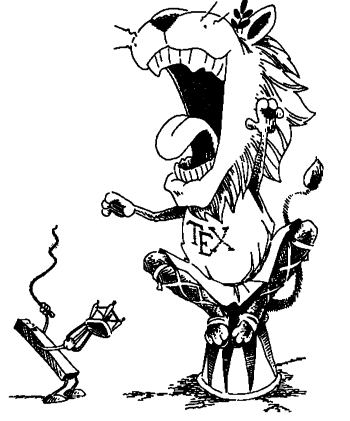
\includegraphics[width = \textwidth]{Chapter3.png}
		\caption{\TeX 的控制系列}\label{subfig:1b}
	\end{subfigure}
	\caption{子图模式测试1:2张图}\label{fig:subfig_test1}
\end{figure}

如\autoref{fig:subfig_test2}是有四张子图的模式,对子图进行交叉引用,如\autoref{subfig:2a}、\autoref{subfig:2b}、\autoref{subfig:2c}和\autoref{subfig:2d}。

\begin{figure}[htbp]
	\centering
	\begin{subfigure}[b]{.4\textwidth}
		\centering
		
\includegraphics[width = \textwidth]{Chapter4.png}
		\caption{字体}\label{subfig:2a}
	\end{subfigure}
	\begin{subfigure}[b]{.4\textwidth}
		\centering
		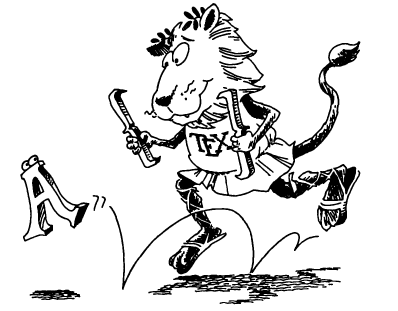
\includegraphics[width = \textwidth]{Chapter5.png}
		\caption{编组}\label{subfig:2b}
	\end{subfigure}
	\begin{subfigure}[b]{.4\textwidth}
		\centering
		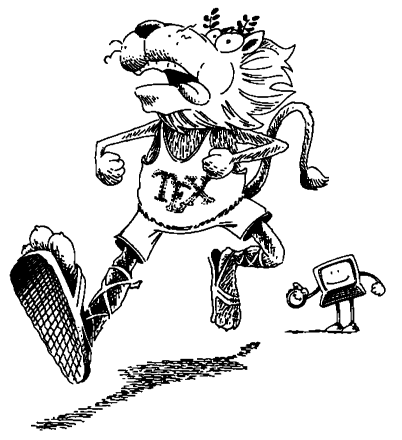
\includegraphics[width = \textwidth]{Chapter6.png}
		\caption{运行\TeX}\label{subfig:2c}
	\end{subfigure}
	\begin{subfigure}[b]{.4\textwidth}
		\centering
		
\includegraphics[width = \textwidth]{Chapter7.png}
		\caption{\TeX 工作原理}\label{subfig:2d}
	\end{subfigure}
	\caption{子图模式测试2:4张图}\label{fig:subfig_test2}
\end{figure}

\subsection{数学模式测试}
数学模式测试,主要测试数学字体,编号和交叉引用。这里首先推荐使用\texttt{align}和\texttt{align*}数学模式环境,大多数行间数学模式只需要用这个环境就可以了。

交叉引用测试,如交引用命令{\ttfamily \textbackslash eqref}和\texttt{\textbackslash ref}命令的区别。如公式\eqref{eq:test1},公式\ref{eq:test1}显示,\texttt{\textbackslash eqref}命令比\texttt{\textbackslash ref}命令的应用结果多了个括号。

如公式\eqref{eq:test3}是单行公式环境,查看公式\eqref{eq:test3}和\eqref{eq:test1}之间的区别,好像在单行公式中没什么区别。
\begin{align}\label{eq:test3}
	f(x) = 2(x + 1)^{2} - 1
\end{align}

\texttt{align}公式环境,用在单行中。
\begin{align}\label{eq:test1}
	f(x) = 2(x + 1)^{2} - 1
\end{align}

在这里,中间插入一些文字以形成段落,查看行间公式与上下文之间的间隙。
\begin{align*}
	f(x) = 2(x + 1)^{2} - 1
\end{align*}
在这里,中间插入一些文字以形成段落,查看行间公式与上下文之间的间隙。下一个公式\eqref{eq:test2}是一个公式组,它在“=”位置对齐。
\begin{align}\label{eq:test2}
	f(x) & = 2(x + 1)^{2} - 1\\
		 & = 2(x^{2} + 2x +1)-1\\
		 & = 2x^{2} + 4x + 1
\end{align}


\section{关于引用}
图表的引用通过{\ttfamily \textbackslash autoref} 命令即可,使用ST LaTeXTools 插件还能自动补全。如果要修改前缀,那么就用{\ttfamily \textbackslash recnewcommand \textbackslash figureautorefname\{好图\}}即可,详见hyperref宏包说明。

\section{出现的问题}
\subsection{\textbackslash texttt}
在这里发现一个问题,在下面的例子中可以发现,在中文中使用\textbackslash texttt\{\}命令时,前面的汉字与接下来的英文单词的空隙明显比接下来单词跟汉字的间隙要大,但是其它命令没有什么问题。

\begin{center}
\noindent 问题\texttt{问题}问题,问题\textbackslash\texttt{问题}问题。\\
问题\texttt{ref} 问题,问题\texttt{\textbackslash ref} 问题。\\
问题\textbf{ref}问题,问题\textbf{\textbackslash ref}问题。\\
问题\textsf{ref}问题,问题\textsf{\textbackslash ref}问题。\\
problem \texttt{ref} problem,problem \texttt{\textbackslash ref} problem.\\
problem \textbf{ref} problem,problem \textbf{\textbackslash ref} problem.\\
problem \textsf{ref} problem,problem \textsf{\textbackslash ref} problem.
\end{center}

原来的编译环境为texlive 2014,编译环境改为texlive 2015后,问题解决。

% !TEX root = ../main.tex
\chapter{学位论文基本结构}
学位论文基本结构包括前置部份、主体部份和结尾部份\footnote{测试脚注另起一章编号的变化}。
\section{前置部分包括}
\begin{enumerate}
	\item 封面
	\item 题名页
	\item 英文题名页(硕士可省略)
	\item 独创性声明(知识产权声明?)
	\item 勘误表(可根据需要)
	\item 致谢
	\item 序言或前沿(可根据需要)
	\item 摘要页
	\item 目次页
	\item 插图和附表清单(可根据需要)
	\item 缩写、符号清单、术语表(可根据需要)
\end{enumerate}
\section{主体部分}
\begin{enumerate}
	\item 引言(绪论)
	\item 正文
	\item 结论
\end{enumerate}
\section{结尾部分}
\begin{enumerate}
	\item 参考文献
	\item 附录(可根据需要)
	\item 索引(根据需要)
	\item 作者简历及在学期间所取得的科研成果
	\item 封底
\end{enumerate}
\chapter{版面设置}
\section{字体设置}
字体设置
\begin{table}[htb]
	\caption{文章字体设置效果}
	\label{tab:文章字体设置效果}
	\begin{center}
		\begin{tabular}{ccc}
			\toprule
					& 英文字体 & 中文字体  \\
			\midrule
			正文字体 & I can eat glass, it doesn't hurt me. & 我能吞下玻璃而不伤身体 \\
			\textbackslash textrm\{\} & \textrm{I can eat glass, it doesn't hurt me.} & \textrm{我能吞下玻璃而不伤身体} \\
			\textbackslash textsf\{\} & \textsf{I can eat glass.} & \textsf{我能吞下玻璃而不伤身体} \\
			\textbackslash texttt\{\} & \texttt{I can eat glass.} & \texttt{我能吞下玻璃而不伤身体} \\
			\textbackslash textbf\{\} & \textbf{I can eat glass.} & \textbf{我能吞下玻璃而不伤身体} \\
			\bottomrule
		\end{tabular}
	\end{center}
\end{table}

% !TEX root = ../main.tex
\chapter{编写规范与要求}
\section{前置部分}
\subsection{封面}
封面包括分类号、密级、单位代码、作者学号、校名、学校徽标、学位论文中文题目、英文题目、作者姓名、导师姓名、学科和专业名称、提交时间等内容(\textbf{见附件1:学位论文封面样式})。
\subparagraph{分类号} % (fold)
\label{par:分类号}
按中国图书分类法,根据学位论文的研究内容确定。
% subparagraph 分类号 (end)
\subparagraph{密级} % (fold)
\label{par:密级}
仅限于涉密学位论文(论文课题来源于国防军工项目)填写,密级应根据涉密学位论文确定,分绝密、机密和秘密三级,并注明保密期限。非涉密学位论文不得填写密级。
% subparagraph 密级 (end)
\subparagraph{单位代码} % (fold)
\label{par:单位代码}
10335
% subparagraph 单位代码 (end)
\subparagraph{作者学号} % (fold)
\label{par:作者学号}
全日制和在职攻读专业学位者填写学号,同等学力申请学位人员填写申请号。
% subparagraph 作者学号 (end)
\subparagraph{论文题目} % (fold)
\label{par:论文题目}
应准确概括整个论文的核心内容,简明扼要,一般不能超过25个汉字,英文题目翻译应简短准确,一般不应超过150个字母,必要时可以加副标题。
% subparagraph 论文题目 (end)
\subparagraph{学科和专业名称} % (fold)
\label{par:学科和专业名称}
必须按国家研究生培养的学科专业目录,规范填写。
% subparagraph 学科和专业名称 (end)
\subsection{题名页} % (fold)
\label{sub:题名页}
题名页应包括:学位论文中英文题目,学位论文导师及作者本人签名,学位论文评阅人姓名、职称和单位等信息(隐名评阅除外),学位论文答辩委员会主席及成员姓名、职称和单位,学位论文答辩日期等(详见附件2题名页样式)。
% subsection 题名页 (end)
\subsection{英文题名页} % (fold)
\label{sub:英文题名页}
中文题名页相对应的英文翻译。
% subsection 英文题名页 (end)
\subsection{独创性声明} % (fold)
\label{sub:独创性声明}
(见附件3浙江大学研究生学位论文独创性声明)。
% subsection 独创性声明 (end)
\subsection{致谢} % (fold)
\label{sub:致谢}
(见附件3浙江大学研究生学位论文独创性声明)。
% subsection 致谢 (end)
\subsection{序言或前言} % (fold)
\label{sub:序言或前言}
学位论文的序言或前言,一般是作者对本篇论文基本特征的简介,如说明研究工作缘起、背景、主旨、目的、意义、编写体例,以及资助、支持、协作经过等。这些内容也可以在正文引言(绪论)中说明。
% subsection 序言或前言 (end)
\subsection{摘要} % (fold)
\label{sub:摘要}
包括中文摘要和英文摘要两部份。摘要是论文内容的总结概括,应简要说明论文的研究目的、基本研究内容、研究方法、创新性成果及其理论与实际意义,突出论文的创新之处。不宜使用公式、图表,不标注引用文献。硕士论文摘要的字数一般为300--500个左右,博士论文摘要的字数为500-1000个。英文摘要应与中文摘要内容相对应。摘要最后另起一行,列出4—8个关键词。关键词应体现论文特色,具有语义性,在论文中有明确的出处。并应尽量采用《汉语主题词表》或各专业主题词表提供的规范词。
% subsection 摘要 (end)
\subsection{目次页} % (fold)
\label{sub:目次页}
论文中内容标题的集合。包括引言(前言)、章节或大标题的序号和名称、小结、参考文献、注释、索引等,排在序言和前言之后另起页(见附件4目次页样式)。
% subsection 目次页 (end)
\subsection{插图和附表清单} % (fold)
\label{sub:插图和附表清单}
论文中如图表较多,可以分别列出清单置于目次页之后。图的清单应有序号、图题和页码。表的清单应有序号、表题和页码。
% subsection 插图和附表清单 (end)
\subsection{缩写、符号清单和术语表} % (fold)
\label{sub:缩写_符号清单和术语表}
符号、标志、缩略词、首字母缩写、计量单位、术语等的注释表。
% subsection 缩写_符号清单和术语表 (end)
\section{主体部份} % (fold)
\label{sec:主体部份}
包括引言(绪论)、正文和结论。主体部分应从另页右页开始,每一章应另起页。
\subsection{一般要求} % (fold)
\label{sub:一般要求}
\subsubsection{引言(绪论)} % (fold)
\label{ssub:引言_绪论_}
应包括论文的研究目的,流程和方法等。论文研究领域的历史回顾,文献回溯,理论分析等内容,应独立成章,用足够的文字叙述。
% subsubsection 引言_绪论_ (end)
\subsubsection{正文} % (fold)
\label{ssub:正文}
主体部分由于涉及不同的学科,在选题、研究方法、结果表达方式等有很大的差异,不能作统一的规定。但是,论文应层次分明、数据可靠、图表规范、文字简炼、说明透彻、推理严谨、立论正确,避免使用文学性质的带感情色彩的非学术性词语。论文中如出现非通用性的新名词、新术语、新概念,应作相应解释。
\subparagraph{图} % (fold)
\label{subp:图}
图应具有“自明性”。图包括曲线图、构造图、示意图、框图、流程图、记录图、地图、照片等,应鲜明清晰。照片上应有表示目的物尺寸的标度。图的编号和图题规范,并应置于图下方。
% subparagraph 图 (end)
\subparagraph{表} % (fold)
\label{subp:表}
表应具有“自明性”。表的编号和表题规范,并置于表上方。表题应简单明了。
表的编排,一般是内容和测试项目由左至右横读,数据依序竖读。如某个表需要转页接排,在随后的各页上应重复表的编号。编号后跟表题(可省略)和“(续)”,置于表上方。续表均应重复表头。
% subparagraph 表 (end)
\subparagraph{公式} % (fold)
\label{subp:公式}
论文中的公式应另行起,并缩格书写,与周围文字留足够的空间区分开。如有两个以上的公式,应用从“1”开始的阿拉伯数字进行编号,并将编号置于括号内。公式的编号右端对齐,公式与编号之间可用“…”连接。公式较多时,应分章编号。较长的公式需要转行时,应尽可能在“=”处回行,或者在“+”、“-”“×”、“/”等记号处回行。
% subparagraph 公式 (end)
\subparagraph{引文标注} % (fold)
\label{subp:引文标注}
论文中引用的文献的标注方法遵照GB/T 7714-2005,可采用顺序编码制,也可采用著者-出版年制,但全文必须统一。如:

德国学者N.克罗斯研究了瑞士巴塞尔市附近侏罗山中老第三纪断裂对第三系摺皱的控制[25];之后,他又描述了西里西亚第3条大型的近南北向构造带,并提出地槽是在不均一的块体的基底上发展的思想[26] 。(顺序编码制)

结构分析的子结构法最早是为解决飞机结构这类大型和复杂结构的有限元分析问题而发展起来的(Przemienicki,1968)(著者-出版年制)
% subparagraph 引文标注 (end)
\subparagraph{注释} % (fold)
\label{subp:注释}
当论文中的字、词或短语,需要进一步加以说明,而又没有具体的文献来源时,用注释。注释一般在社会科学中用得较多。应控制论文中的注释数量,不宜过多。注释采用文中编号加“脚注”的方式,置于当页的页脚。
% subparagraph 注释 (end)
% subsubsection 正文 (end)
% subsection 一般要求 (end)
\subsection{章节图表标号规则} % (fold)
\label{sub:章节图表标号规则}
\subsubsection{章节标号} % (fold)
\label{ssub:章节标号}
论文章节按序分层。层次以少为宜,根据实际需要选择。各层次标题一律用阿拉伯数字连续标号;不同层次的数字之间用小圆点“.”相隔,末位数字后面不加点号,如“1”,“1.1”,“1.1.1”等;章、节编号全部顶格排,编号与标题之间空1个字的间隙。章的标题占2行。正文另起行,前空2个字起排,回行时顶格排。例如:
\begin{verbatim}
1 ××××(章大标题),
×××××××××××××××××××××××××××
1.1 ××××(一级节标题)
1.1.1 ××××(二级节标题)
1.1.1.1 ××××(根据需要,也可设三级节标题)
2 ××××(章大标题)
2.1 ××××(一级节标题)
2.1.1 ××××(二级节标题)
\end{verbatim}
% subsubsection 章节标号 (end)
\subsubsection{图、表等标号} % (fold)
\label{ssub:图_表等标号}
论文中的图、表、附注、公式、算式等,一律用阿拉伯数字分章依序连续编码。其标注形式应便于互相区别,如:图 l.1(第1章第一个图)、图2.2(第二章第二个图);表3.2(第三章第二个表)等。
% subsubsection 图_表等标号 (end)
\subsubsection{页码、页眉编写规则} % (fold)
\label{ssub:页码_页眉编写规则}
学位论文的页码,前置部分用罗马数字单独编连续码,正文和后置部分用阿拉伯数字编连续码。单面复印时页码排在页脚居中位置,双面复印时页码分别按左右侧排列。

页眉、页脚文字均采用小五号宋体,左侧页眉为“浙江大学博(硕)士学位论文”,右侧为一级标题名称;页眉下横线可为单横线也可用上粗下细文武线。
% subsubsection 页码_页眉编写规则 (end)
% subsection 章节图表标号规则 (end)
\subsection{结论} % (fold)
\label{sub:结论}
论文的结论是最终的、总体的结论,不是正文中各段的小结的简单重复。结论应包括论文的核心观点,交代研究工作的局限,提出未来工作的意见或建议。结论应该准确、完整、明确、精练。

如果不能导出一定的结论,也可以没有结论而进行必要的讨论。
% subsection 结论 (end)
% section 主体部份 (end)
\section{结尾部分} % (fold)
\label{sec:结尾部分}
\subsection{参考文献} % (fold)
\label{sub:参考文献}
参考文献表是文中引用的有具体文字来源的文献集合,其著录项目和著录格式遵照GB/T 7714-2005的规定执行。

参考文献表应置于正文后,并另起页。所有被引用文献均要列入参考文献表中。引文采用顺序编码标注时,参考文献表按编码顺序排列,引文采用著作-出版年制标注时,参考文献表应按著者字顺和出版年排序。

各种主要参考文献按如下格式编排:

学术期刊:序号 作者 文题 刊名 年 卷号(期号) 起止页码

专(译)著:序号 作者(译者) 书名. 出版地:出版者,出版年,起止页码

学位论文:序号 作者 文题 [XX学位论文] 授予单位所在地 授予单位 授予年份  起止页码

专利:序号 申请者 专利名 国名 专利文献种类 专利号 出版日期

技术标准:序号 发布单位 技术标准代号 技术标准名称 出版地:出版者,出版日期

电子文献:序号 作者 出版年 题名 出版地 出版者 [引用日期] 获取和访问路径
% subsection 参考文献 (end)
\subsection{附录} % (fold)
\label{sub:附录}
附录作为主体部分的补充,并不是必须的。

下列内容可以作为附录编于论文后。

为了整篇论文材料的完整,但编入正文又有损于编排的条理性和逻辑性,这一材料包括比正文更为详尽的信息、研究方法和技术更深入的叙述,对了解正文内容有用的补充信息等。

由于篇幅过大或取材于复制品而不便于编入正文的材料。

不便于编入正文的罕见珍贵资料。

对一般读者并非必要阅读,但对本专业同行有参考价值的资料。

某些重要的原始数据、数学推导、结构图、统计表、计算机打印输出件等。
% subsection 附录 (end)
\subsection{索引} % (fold)
\label{sub:索引}
根据需要可以编排分类索引,关键词索引等。
% subsection 索引 (end)
\subsection{作者简历} % (fold)
\label{sub:作者简历}
包括教育经历、工作经历、攻读学位期间发表的论文和完成的工作等。
% subsection 作者简历 (end)
% section 结尾部分 (end)

\backmatter
\bibliography{reference_data_base/MyMasterThesisReferences}
% \nocite{*} % to show the entire references, annotate it if need.
\appendix
% !TEX root = ../main.tex
\chapter{我是第一个附录}
\section{我是第一个附录的第一节}
这是一个附录测试页,内容无关紧要。\footnote{以下内容引用自《三体:黑暗森林》}以%
下段落较长,以防数组溢出,故采用回车强制分行处理。分行出换行符在\TeX 中算作一个%
空格,因此,在每段后加注释符。不过在中文环境中换行加不加注释符都不会产生空格,不%
过还是加上吧。

罗辑抬起左手,露出了戴在手腕上的手表大小的东西说:“这是一个生命体征监测仪,它通%
过一个发射器与一套摇篮系统联结。你们一定记得两个世纪前面壁者雷迪亚兹的事,那就一%
定知道摇篮系统是什么。这个监测仪所发出的信号通过摇篮系统的链路,到达雪地工程部署%
在太阳轨道上的三千六百一十四枚核弹。

信号每秒钟发射一次,维持着这些核弹的非触发状态。如果我死去,摇篮系统的维持信号将%
消失,所有的核弹将被引爆,包裹核弹的油膜物质将在爆炸中形成围绕太阳的三千六百一十%
四团星际尘埃,从远方观察,在这些尘埃云团的遮挡下,太阳将在可见光和其他高频渡段发%
生闪烁。太阳轨道上所有核弹的位置都是经过精心布置的,使得太阳闪烁形成的信号发送出%
三张简单的图形,就像我两个世纪前发出的那三张图一样,每张上面有三十个点的排列,并%
标注其中一个点,它们可以组合成一个三维坐标图。但与那次不同的是,这次发送的,是三%
体世界与周围三十颗恒星的相对位置。太阳将变成银河系中的一座灯塔,把这咒语发送出去%
,当然,太阳系和地球的位置也会同时暴露。从银河系中的一点看,图形发射完成需要一年%
多的时间,但应该有很多技术发展到这样程度的文明,可以从多个方向同时观测太阳,那样%
的话,只需几天甚至几个小时,他们就能得到全部信息。”

\section{数学模式测试}
这里用于测试附录部分的数学公式,诸如标号,交叉应用等。

交叉引用测试,如交引用命令{\ttfamily \textbackslash eqref}和\texttt{\textbackslash ref}命令的区别。如公式\eqref{eq:apptest1},\autoref{eq:apptest1}显示,\texttt{\textbackslash eqref}命令比\texttt{\textbackslash ref}命令的应用结果多了个括号。

如公式\eqref{eq:apptest3}是单行公式环境,查看公式\eqref{eq:apptest3}和\eqref{eq:apptest1}之间的区别,好像在单行公式中没什么区别。
\begin{align}\label{eq:apptest3}
	f(x) = 2(x + 1)^{2} - 1
\end{align}

\texttt{align}公式环境,用在单行中。
\begin{align}\label{eq:apptest1}
	f(x) = 2(x + 1)^{2} - 1
\end{align}

在这里,中间插入一些文字以形成段落,查看行间公式与上下文之间的间隙。
\begin{align*}
	f(x) = 2(x + 1)^{2} - 1
\end{align*}
在这里,中间插入一些文字以形成段落,查看行间公式与上下文之间的间隙。下一个公式\eqref{eq:apptest2}是一个公式组,它在“=”位置对齐。
\begin{align}\label{eq:apptest2}
	f(x) & = 2(x + 1)^{2} - 1\\
		 & = 2(x^{2} + 2x +1)-1\\
		 & = 2x^{2} + 4x + 1
\end{align}

\subsection{我是第一个附录的第二节的第一个子节}

\section{表格测试}
在这里推荐制表采用功能强大的tabu宏包以取代其它制表宏包。具体tabu宏包的使用说明参见tabu宏包的说明文档。

以下节分别用来测试各种表格环境如,tabular,tabu,longtabu等,还有对caption格式的修改和测试。以下表格样式全部采用三线表。

\subsection{array宏包tabular表格环境测试}
如\autoref{tab:appfirst_table_test}是对array宏包的tabular表格环境测试。
\begin{table}[htbp]
	\centering
	\caption{这是一个用tabular环境的测试用的表格}\label{tab:appfirst_table_test}
    \begin{tabular}{lrr}
    \toprule
    \textbf{行星}     & \textbf{赤道半径}km & \textbf{公转周期}d \\
    \midrule
    水星     & 2.439  & 87.9 \\
    金星     & 6.1    & 224.682 \\
    地球     & 6378.14 & 365.24 \\
    \bottomrule
    \end{tabular}%
\end{table}

\subsection{tabu宏包表格环境测试}
如\autoref{tab:apptabu_test_1}是对tabu宏包的tabu表格环境测试。在这里表格命令与\autoref{tab:appfirst_table_test}的命令相同,只是tabular环境改成了tabu环境。
\begin{table}[htbp]
	\centering
	\caption{这是一个用tabu环境的测试用的表格}\label{tab:apptabu_test_1}
    \begin{tabu}{lrr}
    \toprule
    \textbf{行星}     & \textbf{赤道半径}km & \textbf{公转周期}d \\
    \midrule
    水星     & 2.439  & 87.9 \\
    金星     & 6.1    & 224.682 \\
    地球     & 6378.14 & 365.24 \\
    \bottomrule
    \end{tabu}%
\end{table}

\section{插图测试}
如\autoref{fig:appfirst_image_tset}是对此模版的第一张插图测试。

\begin{figure}[htbp]
	\centering
	
\includegraphics[width = 0.5\linewidth]{Chapter8.png}
	\caption{附录页第一张插图测试}\label{fig:appfirst_image_tset}
\end{figure}

\section{我是第一个附录的第五节}
随着天光渐明,星星在一颗颗消失,仿佛无数只眼睛渐次闭上;而东方正在亮起的晨空,则%
像一只巨大的眼睛在慢慢睁开。蚂蚁继续在叶文洁的墓碑上攀爬着,穿行在她的名字构成的%
迷宫中。早在这个靠碑而立的豪赌者出现前的一亿年,它的种族已经生活在地球上,这个世%
界有它的一份,但对正在发生的事,它并不在意。

罗辑离开墓碑,站到他为自己挖掘的墓穴旁,将手枪顶到自己的心脏位置,说:“现在,我
将让自己的心脏停止跳动,与此同时我也将成为两个世界有史以来最大的罪犯。对于所犯下
的罪行,我对两个文明表示深深的歉意,但不会忏悔,因为这是唯一的选择。我知道智子就
在身边,但你们对人类的呼唤从不理睬,无言是最大的轻蔑,我们忍受这种轻蔑已经两个世
纪了,现在,如果你们愿意,可以继续保持沉默,我只给你们三十秒钟时间。”罗辑按照自
己的心跳来计时,由于现在心跳很急促。他把两次算一秒钟,在极度的紧张中他一开始就数
错了,只好从头数起,所以当智子出现时他并不能确定到底过了多少时间,客观时间大约流
逝了不到十秒钟,主观时间长得像一生。

这时他看到世界在眼前分成了四份,一份是周围的现实世界,另外三份是变形的映像。映像%
来自他前上方突然出现的三个球体,它们都有着全反射的镜面,就像他在最后一个梦中见到%
的墓碑那样。他不知道这是智子的几维展开,那三个球体都很大,在他的前方遮住了半个天%
空,挡住了正在亮起来的东方天际,在球体中映出的西方天空中他看到了几颗残星,球体下%
方映着变形的墓地和自己。罗辑最想知道的是为什么是三个,他首先想到的是三体世界的象%
征,就像叶文洁在最后一次ETO的聚会上看到的那个艺术品:但看到球体上所映照的虽然变%
形但异常清晰的现实图像时,他又感觉那是三个平行世界的入口,暗示着三种可能的选择;

% !TEX root = ../main.tex
\chapter{我是第二个附录}
\section{我是第二个附录的第一节}
这是一个附录测试页,内容无关紧要。\footnote{以下内容引用自《三体:死神永生》}

这时。“蓝色空间”号和“万有引力”号同时停止前进,并后退了三十万千米,因为“魔戒”进入%
三维太空时,在维度跌落过程中将放出巨大的能量,这也是之前出现的那些长线发光的原因。%

二十二天后,四维碎块的边界退过了“魔戒”。在它进入三维太空的那一瞬间,宇宙仿佛被拦%
腰斩断,长长的断口发出炫目的强光,如同一颗恒星被瞬间拉成一条线。当光芒黯淡一些后%
,一条横过整个太空的长线显现出来,从飞船上看不到它的头和尾,像上帝在宇宙的绘图板%
上比着丁字尺从左到右画了一道。据测量,这条把可见的宇宙分成两部分的线,其长度接近%
一个天文单位。约一亿三千万千米,几乎可以把地球和太阳连接起来。与以前出现的那些长%
线不同,这条线即使从几十万千米外仍能看出其宽度。长线发出的光由蓝白变成红色,然后%
渐渐暗淡下去,线本身也变得宽散弯曲。由一条笔直的长线变成一道尘埃带,弯弯曲曲不见%
首尾。它自身己经不发光,但浸透了星海的光芒,变成宁静的银灰色。两艘飞船上观看的人%
们这时都有一个奇怪的印象,感觉尘埃带看上去很像宇宙背景上的银河系,刚才发生的仿佛%
是一次对银河系的宏大摄影,闪光灯闪过后,拍下的照片在太空中渐渐显影。

看着这壮丽的景象,关一帆有些伤感,他想起了自己送给“魔戒”的生态球,它只拥有了那个%
礼物不长的时间。在三维展开的一刹那,“魔戒”内部的所有四维结构都被完全破坏,这是一%
场最彻底的毁灭。四维碎块中其他那些已经死去或仍活着的飞船,最终也都无法逃脱这样的%
命运,在这广阔的宇宙中,它们只能在四维碎块这个小小的角落中存在。

一个巨大而黑暗的秘密。

“蓝色空间”号和“万有引力”号派出多艘太空艇前往尘埃带,除了考察外,还想看看能不能收%
集一些有用的资源。“魔戒”三维化以后都变成很普通的元素,大部分是氢和氮,从中有可能%
得到核聚变燃料。但尘埃中的这两种元素都呈气态,扩散很快,没有收集到多少。另外还有%
一些重元素。可以采集到一些有用的金属。

现在,两艘飞船应该考虑自己的未来了。由“蓝色空间”号和“万有引力”号共同组成的一个临%
时委员会宣布,两艘飞船上的任何人都可以做出选择:随两舰继续航行或返回太阳系。两舰%
将装配一个独立于两舰的冬眠舱,并把两舰上七台聚变发动机中的一台用于推进它,决定返%
回的人将乘坐这艘临时装配的飞船,在冬眠中返回太阳系,航行时问预计为三十五年。两舰%
将用中微子通信通知地球冬眠飞船的轨道参数,以便在它到达太阳系时进行接应。为了防止%
三体世界借此侦测到两舰的位置,与地球的联系将在冬眠飞船起航一段时间后再进行。如果%
地球方面能够在飞船到达太阳系前派出接应飞船协助减速的话,加速段就有更多的燃料用于%
推进,返回的航程可以缩短至十几年。

如果那时还有太阳系和地球的话。

只有两百多人选择返回,其余的人不想回到那个正在走向毁灭的世界,决定随“蓝色空间”号%
和“万有引力”号继续航行,飞向未知的太空深处。

\subsection{我是第二个附录的第一节的第一个子节}
\subsubsection{我是第二个附录的第一节的第一个子节的第一个子子节}

\end{document}